% \newpage
\subsection{Управление качеством}
\label{bp:quality}
%\subsection{Управление качеством}

На ПРЕДПРИЯТИИ создан Отдел Управления Качеством. 
%(далее ОУК). 

\subsubsection{Работа контролеров на производстве} 

В начале каждой смены контролеры ОУК открывают и распечатывают из системы 1С: УПП сменное задание (рис. \ref{pic:/VIIIзадание}). Машинисты гофроагрегата и машинисты линий переработки предоставляют контролерам ОУК образцы с каждого задания, контролеры ОУК проводят лабораторные испытания предоставленных образцов. 

На линиях переработки машинисты и контролеры ОУК совместно заполняют печатный бланк ''Лист контроля качества изделия''. Контролеры ОУК оформляют в системе 1С: УПП ''Протокол испытаний'' (рис. \ref{pic:/VIIIрезультатыиспытаний}), информацию дублируют в журналы (рис. \ref{pic:/VIII Задание и журнал}). В результате в системе 1С: УПП формируется статистика и есть возможность сформировать различные отчеты по качеству продукции (рис. \ref{pic:/VIIIотчет1}, \ref{pic:/VIIIотчет2},\ref{pic:/VIIIотчет3}).  

В случае выявления брака техник по качеству оформляет в системе 1С: УПП акт (рис. \ref{pic:/VIII.11.}). Брак хранится в специальном отведенном месте (рис. \ref{pic:/VIII как хранить брак}).

Брак листового картона и выпущенных на ГА полуфабрикатов  используется для упаковки готовой продукции. 

На ПРЕДПРИЯТИИ создан склад хранения эталонных образцов ГП (рис. \ref{pic:/VIIIконтрольныеобразцы}). На ПРЕДПРИЯТИИ существует практика сверки выпускаемой продукции с эталонными образцами, утвержденными заказчиками.


\subsubsection{Приемка сырья} 

Приемка сырья представителями ОУК производится при поступлении рулонов с АО ''АЦБК'' и АО ''СЛПК''. Производится осмотр рулонов и выполняются лабораторные испытания образцов. По итогам проведения испытаний оформляется ''Протокол испытаний'' (рис. \ref{pic:/VIII.1}) в системе 1С: УПП. Дополнительно информация дублируется в журналах (рис. \ref{pic:/VIII анализы сырья}).
Приемка рулонов ООО ''ПЗБМ'' ОУК не производится, но в случае выявления проблем производится запрос  о предоставлении информации по рулонам. 
% (рис. \ref{pic:/VIII.6}).


\subsubsection{Внутренние претензии}

Создание и рассмотрение внутренних претензий производится ОУК. Внутренние претензии оформляются в  системе 1С: УПП при выявлении брака на различных рабочих центрах (рис. \ref{pic:/VIII.11}). На основании информации в системе  1С: УПП в MS Excel формируются отчеты по внутренним претензиям (рис. \ref{pic:/VIIIвнпретензии}).

\subsubsection{Контроль материалов}

В лаборатории каждую  смену производится анализ параметров клея на гофроагрегате. Результаты фиксируются в журнале ''Контроля по вязкости''  (рис. \ref{pic:/VIII журнал клея}). Замеры ''сухого остатка'' производятся только в дневные смены. Отчеты по замерам формируются в MS Excel (рис. \ref{pic:/VIIIсухойостаток}).
%Контролер ОТК сводит итоговый отчет в сводную таблицу для вывода данных на монитор в цеху (рис. \ref{pic:a16}).


\subsubsection{Лаборатория}

На ПРЕДПРИЯТИИ создана лаборатория. Лаборатория аттестована. Приборы проходят регулярные поверки (рис. \ref{pic:/VIIIлаборатория}). 

\subsubsection{Отчеты по качеству}

На основе информации из системы 1С: УПП формируются  отчеты и презентация по качеству и претензиям (рис. \ref{pic:/VIIIкачество}). Имеется возможность ознакомиться с информацией по сырью и выработкой продукции и дать ответ на претензии клиентов. Ежегодно определяются и реализуются мероприятия по снижению количества некондиционной продукции (рис. \ref{pic:/VIIIсовещание}).  
  
%На несколько заказов приказом по предприятию (рис. \ref{pic:a18}) допускается повышенный брак из-за сложности при производстве.

%ОТК составляет сводный отчет по дням (рис. \ref{pic:a20}).

%На предприятии выделена лаборатория. 

%В лабораторию поступает задание на ГА. Лаборант берет заготовку и проводит лабораторные испытания. Лаборант измеряет показатель ЕСТ и толщину заготовки. Результаты измерений лаборант заносит на форму задания (рис. \ref{pic:f38}) и в журнал (рис. \ref{pic:f40}). 
%При значительном отклонении значений показателей от норм лаборант составляет акт и заносить показатели в журнал показателей.\
% (рис. \ref{pic:f40}).


%На перерабатывающих линиях лаборант измеряет показатель качества ЕСТ и толщину картона, проверяет геометрию и печать. Разработаны образцы недочетов, на которые можно не обращать внимание при проведении контроля качества продукции (рис. \ref{pic:f42}).

%По просьбе главного технолога лаборанты проводят измерение влажности на образцах сырья, поступившего на производство (рис. \ref{pic:f41}). Входящее сырье на склад не контролируется службой ОТК.

%акже по просьбе менеджеров лаборанты определяют состав образцов от клиента и марку.
%При поступлении заготовки в цех контролер ОТК проверяет заготовки на механические повреждения и при выявлении брака составляет акт и делает фото (рис. \ref{pic:a64}). Претензии к поставщику контролер ОТК выставляет при превышении количества брака более чем на 2 процента от общего объема поставки.

%Далее контролер ОТК начинает претензионную работу: отправляет претензию и ожидает ответа от поставщика. После прихода письма от поставщика 
% (рис. \ref{pic:a59}) 
%и при появлении представителей поставщика контролер ОТК собирает комиссию и составляет акт отбраковки (рис. \ref{pic:a60}). 

%Если продукция подлежит возврату, контролер ОТК составляет акт выбраковки и сопроводительные документы (рис. \ref{pic:a61}, рис. \ref{pic:a62}).

%Претензии от покупателей по готовой продукции поступают менеджерам.
%При появлении претензии от покупателя на ГП менеджеры стараются решить на месте. Документы по претензиям от потребителей не ведутся. 

%На линии контролер ОТК проверяет размеры, качество печати и толщину картона толщиномером.
%Контролер ОТК ведет журнал измерения толщины по номенклатуре выпускаемых изделий (рис. \ref{pic:a63}).
\clearpage
\begin{figure}
\begin{center}
 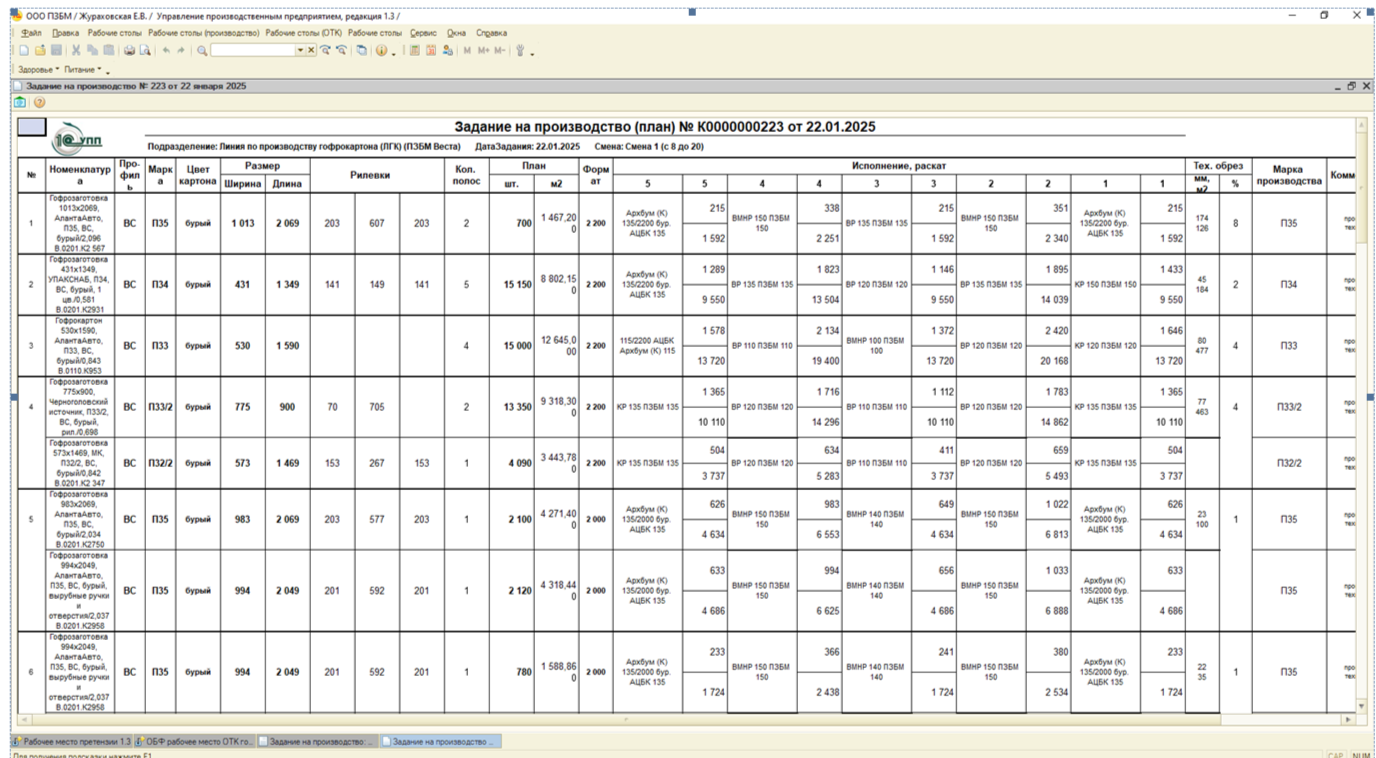
\includegraphics[height=0.45\textheight, angle=90, keepaspectratio]{Pics/VIIIзадание.png}
\end{center}
 \caption{Плановое задание}
 \label{pic:/VIIIзадание}
\end{figure}

\begin{figure}
\begin{center}
 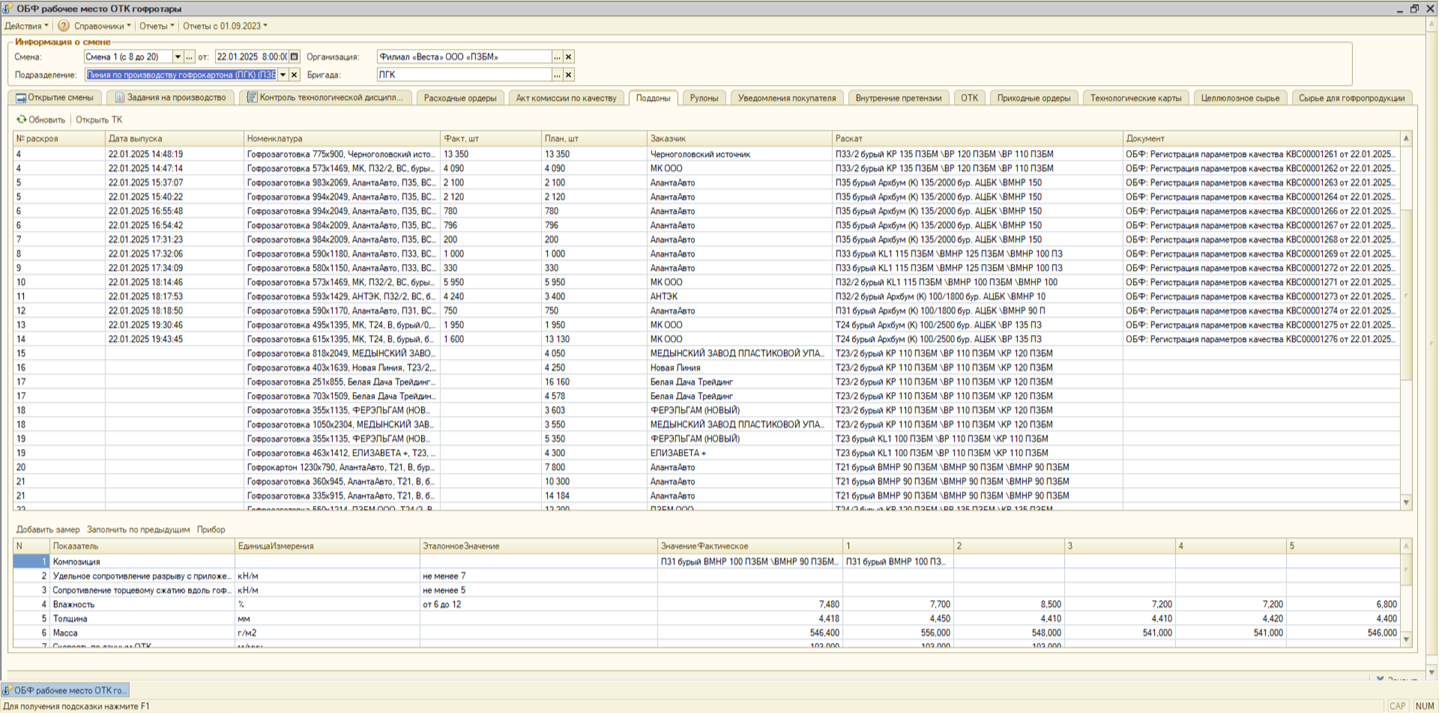
\includegraphics[height=0.45\textheight, angle=90, keepaspectratio]{Pics/VIIIрезультатыиспытаний.png}
\end{center}
 \caption{Результаты лабораторных испытаний}
 \label{pic:/VIIIрезультатыиспытаний}
\end{figure}

\begin{figure}
\begin{center}
 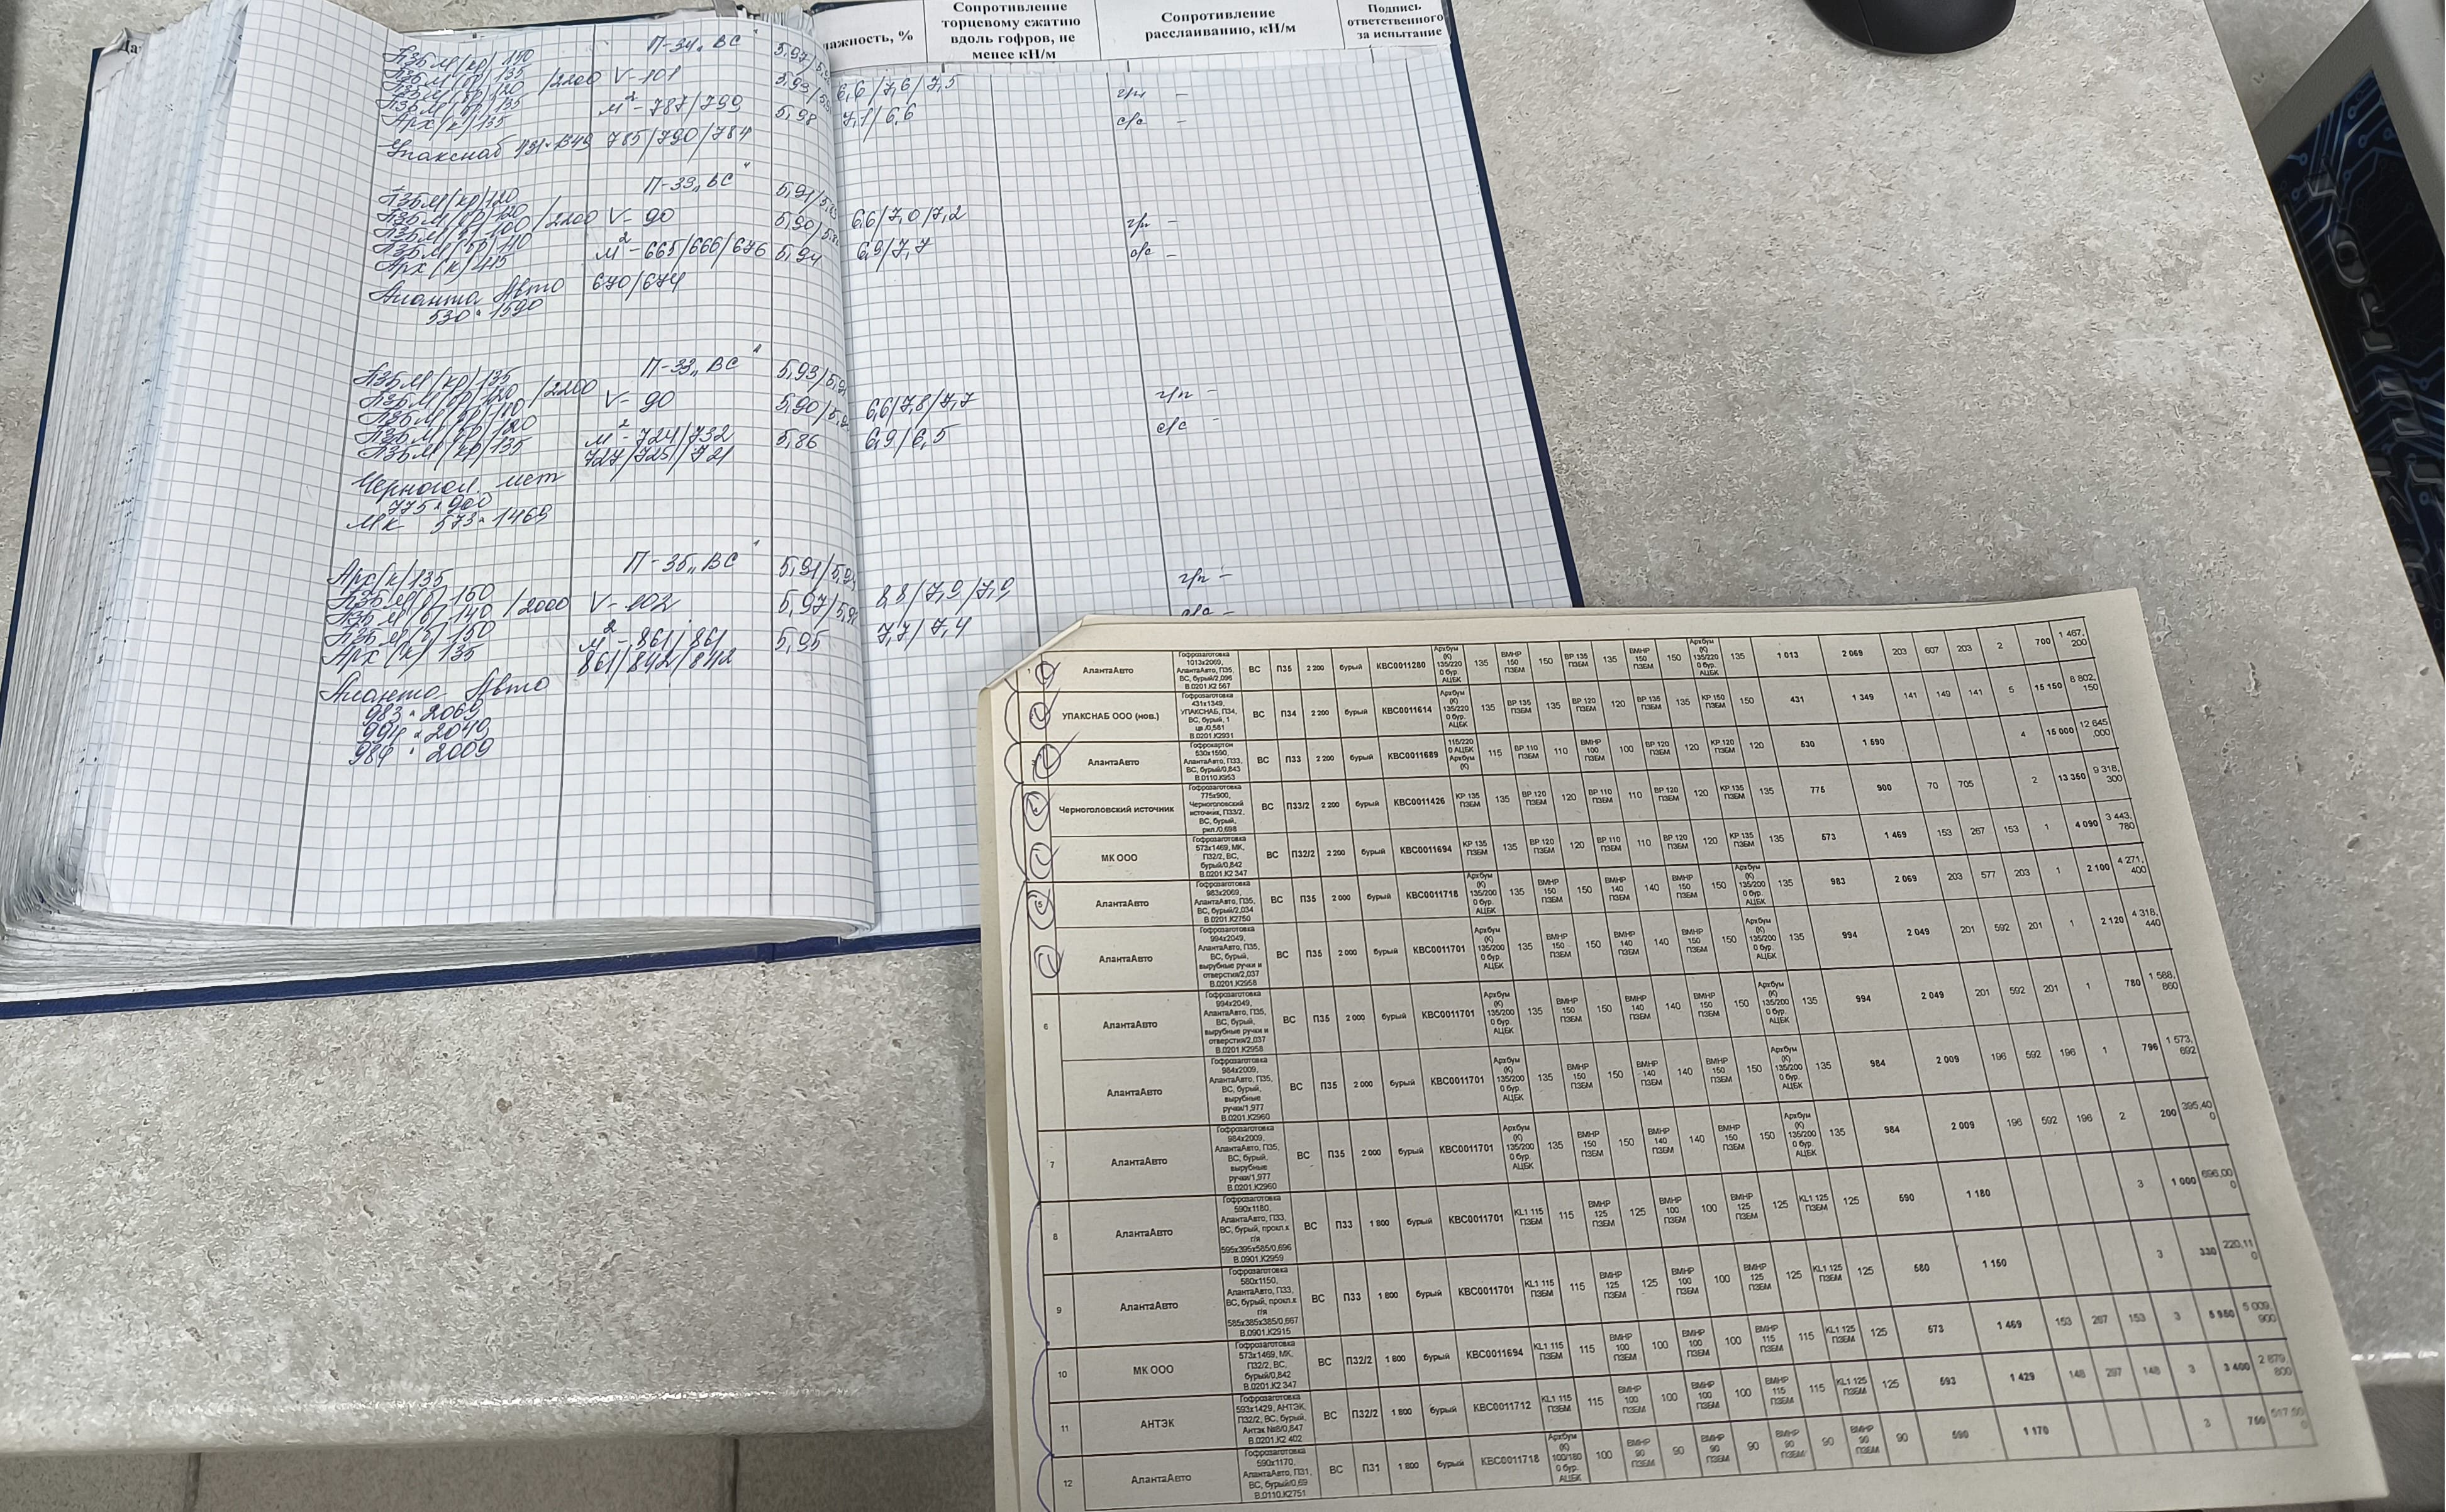
\includegraphics[height=0.4\textheight, keepaspectratio]{Pics/VIII Задание и журнал.jpg}
\end{center}
 \caption{Результаты лабораторных испытаний}
 \label{pic:/VIII Задание и журнал}
\end{figure}

\begin{figure}
\begin{center}
 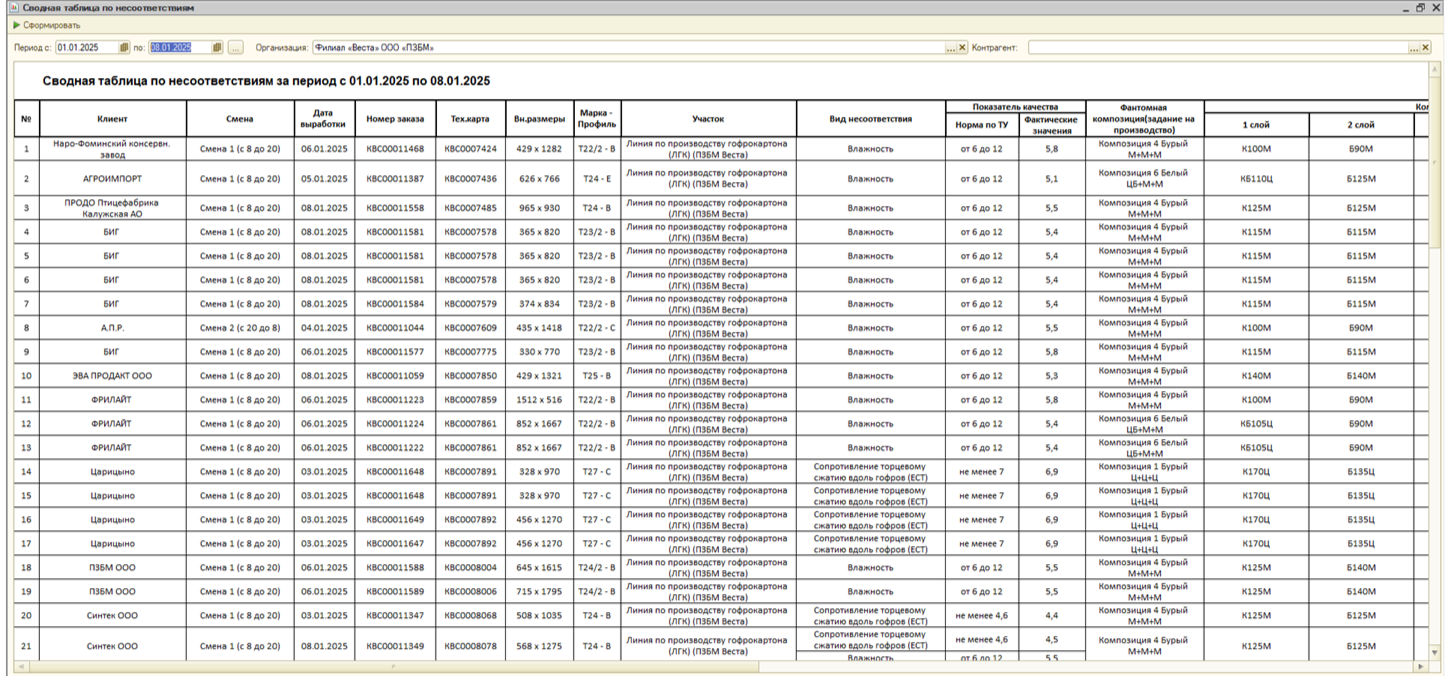
\includegraphics[height=0.3\textheight, keepaspectratio]{Pics/VIIIотчет1.png}
\end{center}
 \caption{Отчеты в системе 1С: УПП}
 \label{pic:/VIIIотчет1}
\end{figure}

\begin{figure}
\begin{center}
 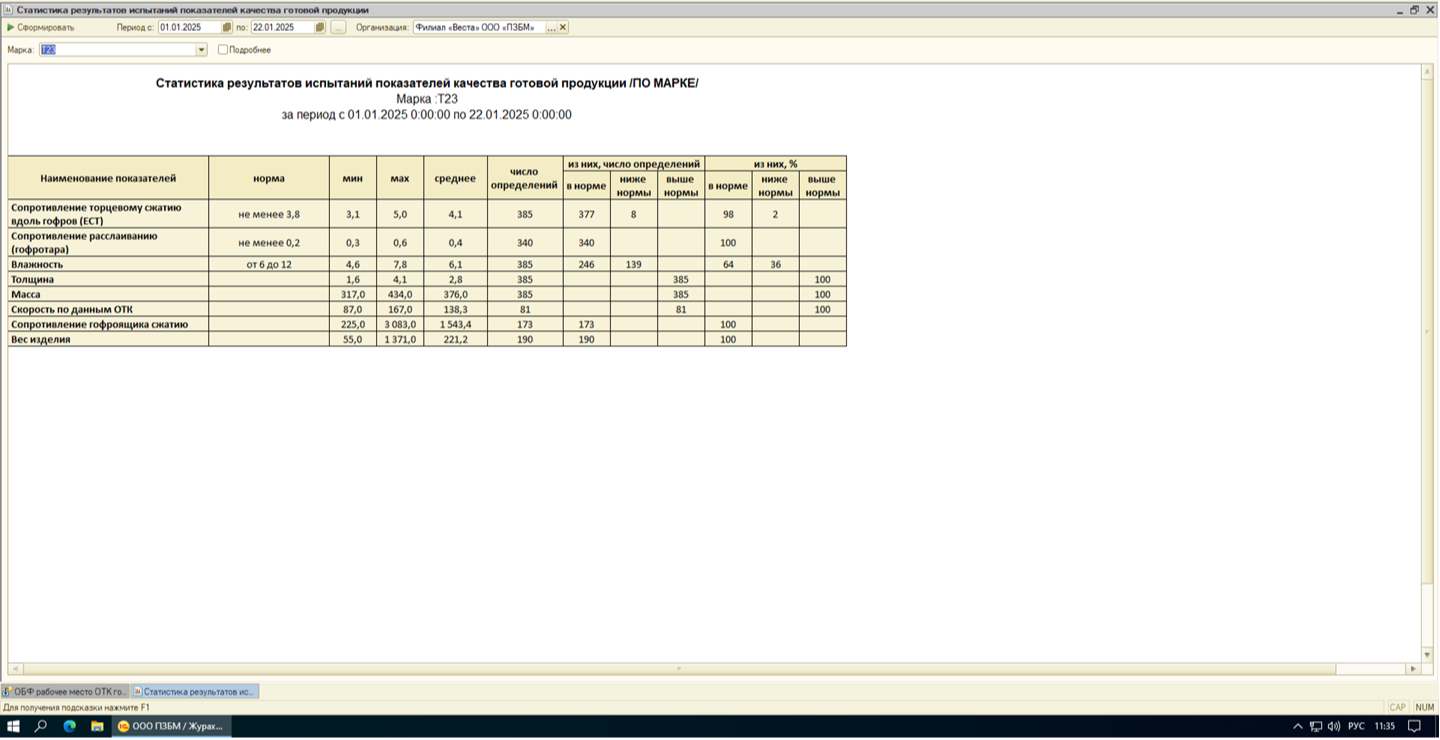
\includegraphics[height=0.3\textheight, keepaspectratio]{Pics/VIIIотчет2.png}
\end{center}
 \caption{Отчеты в системе 1С: УПП}
 \label{pic:/VIIIотчет2}
\end{figure}

\begin{figure}
\begin{center}
 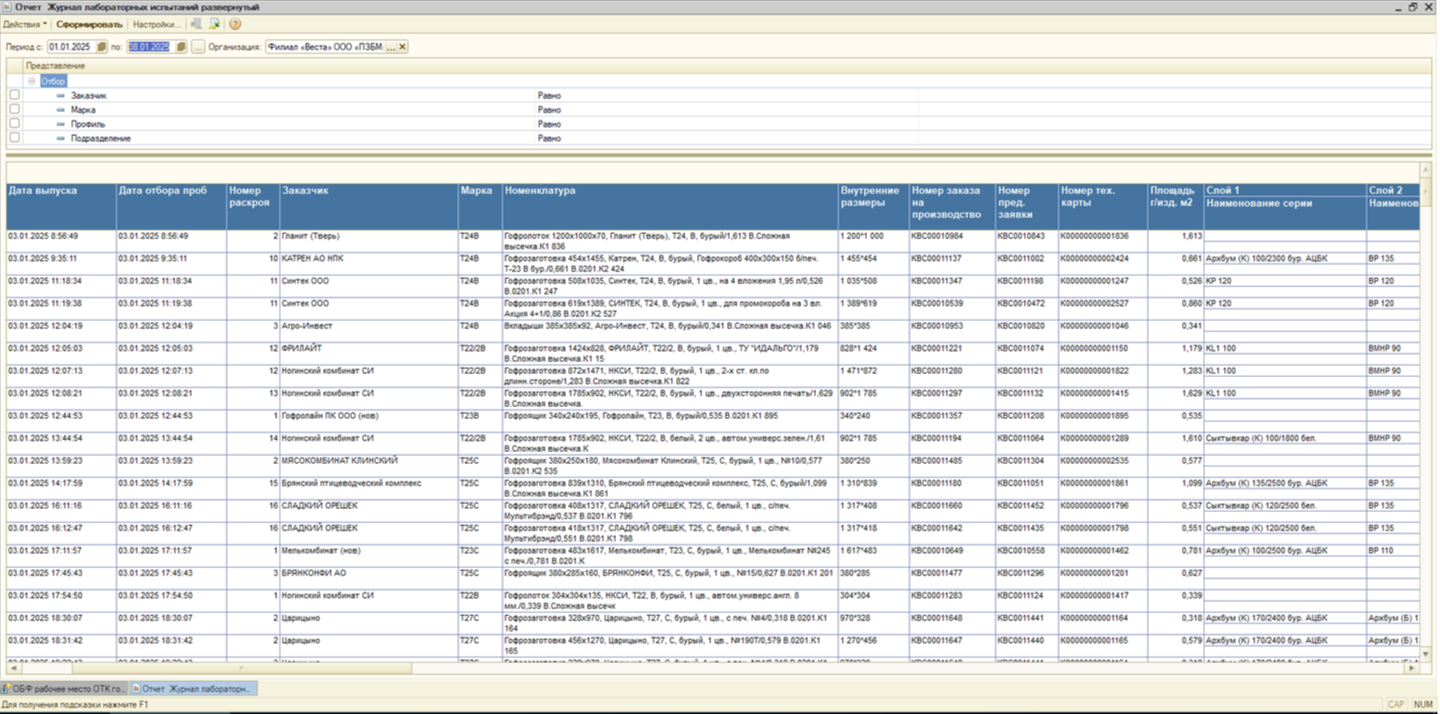
\includegraphics[height=0.3\textheight, keepaspectratio]{Pics/VIIIотчет3.png}
\end{center}
 \caption{Отчеты в системе 1С: УПП}
 \label{pic:/VIIIотчет3}
\end{figure}

\begin{figure}
\begin{center}
 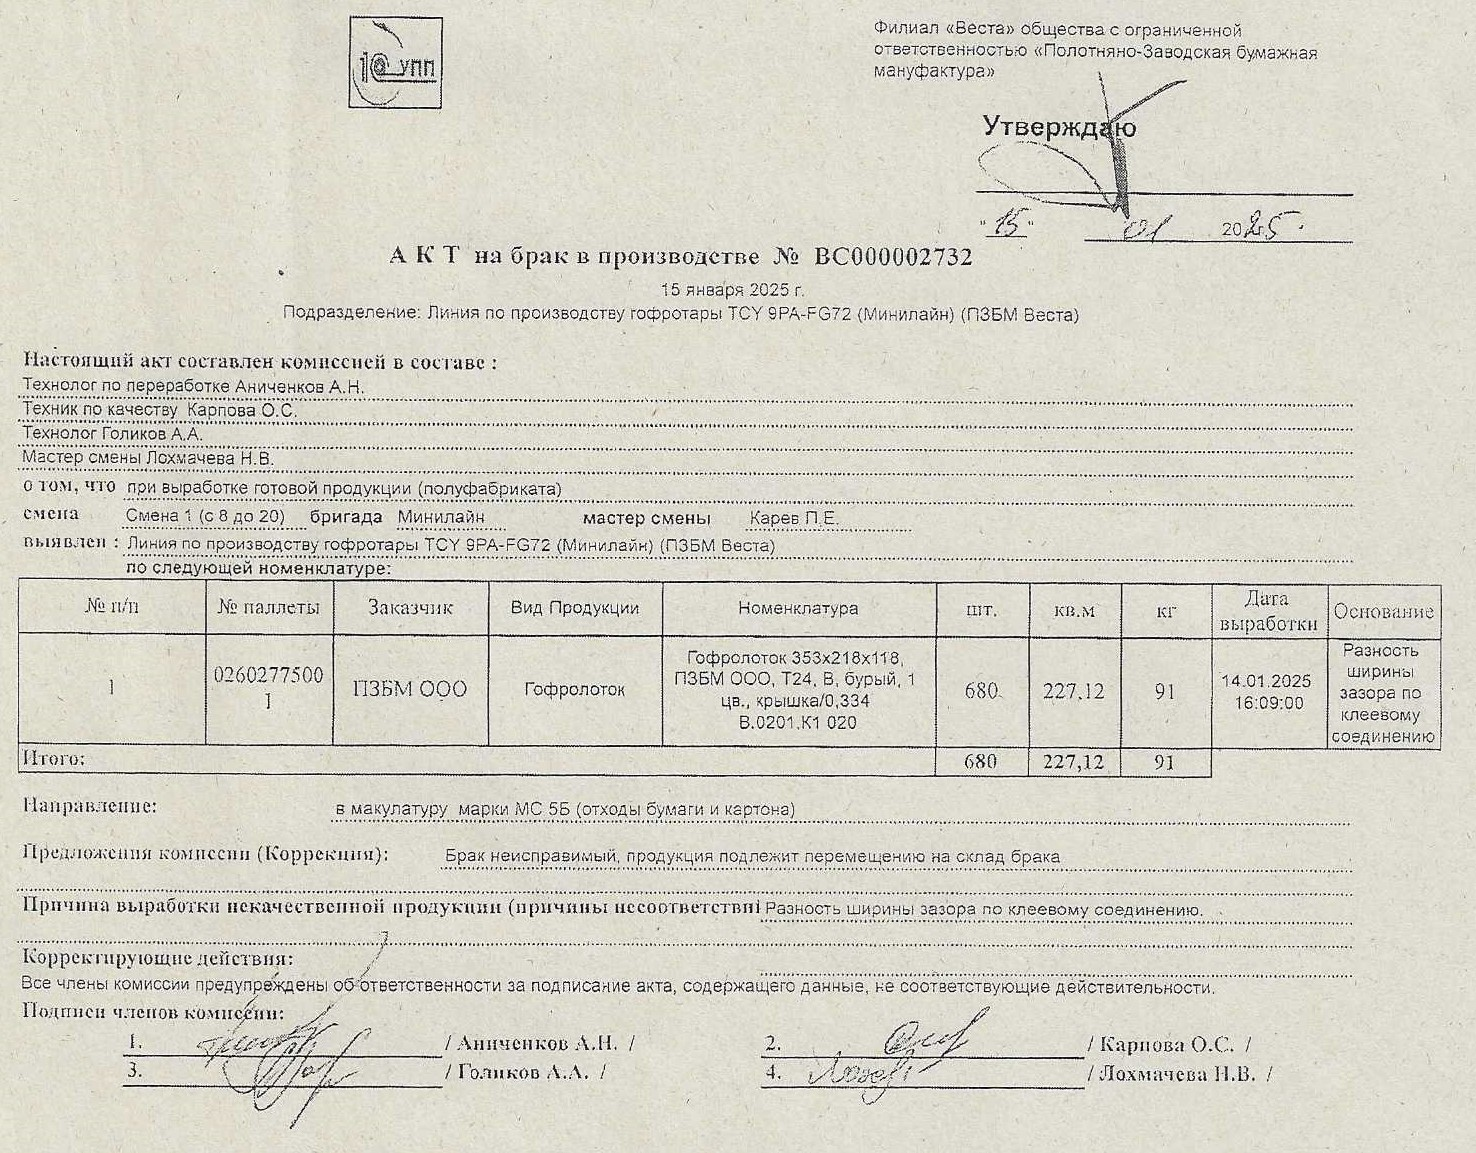
\includegraphics[height=0.5\textheight, keepaspectratio]{Pics/VIII.11..jpg}
\end{center}
 \caption{Акт на брак}
 \label{pic:/VIII.11.}
\end{figure}

\begin{figure}
\begin{center}
 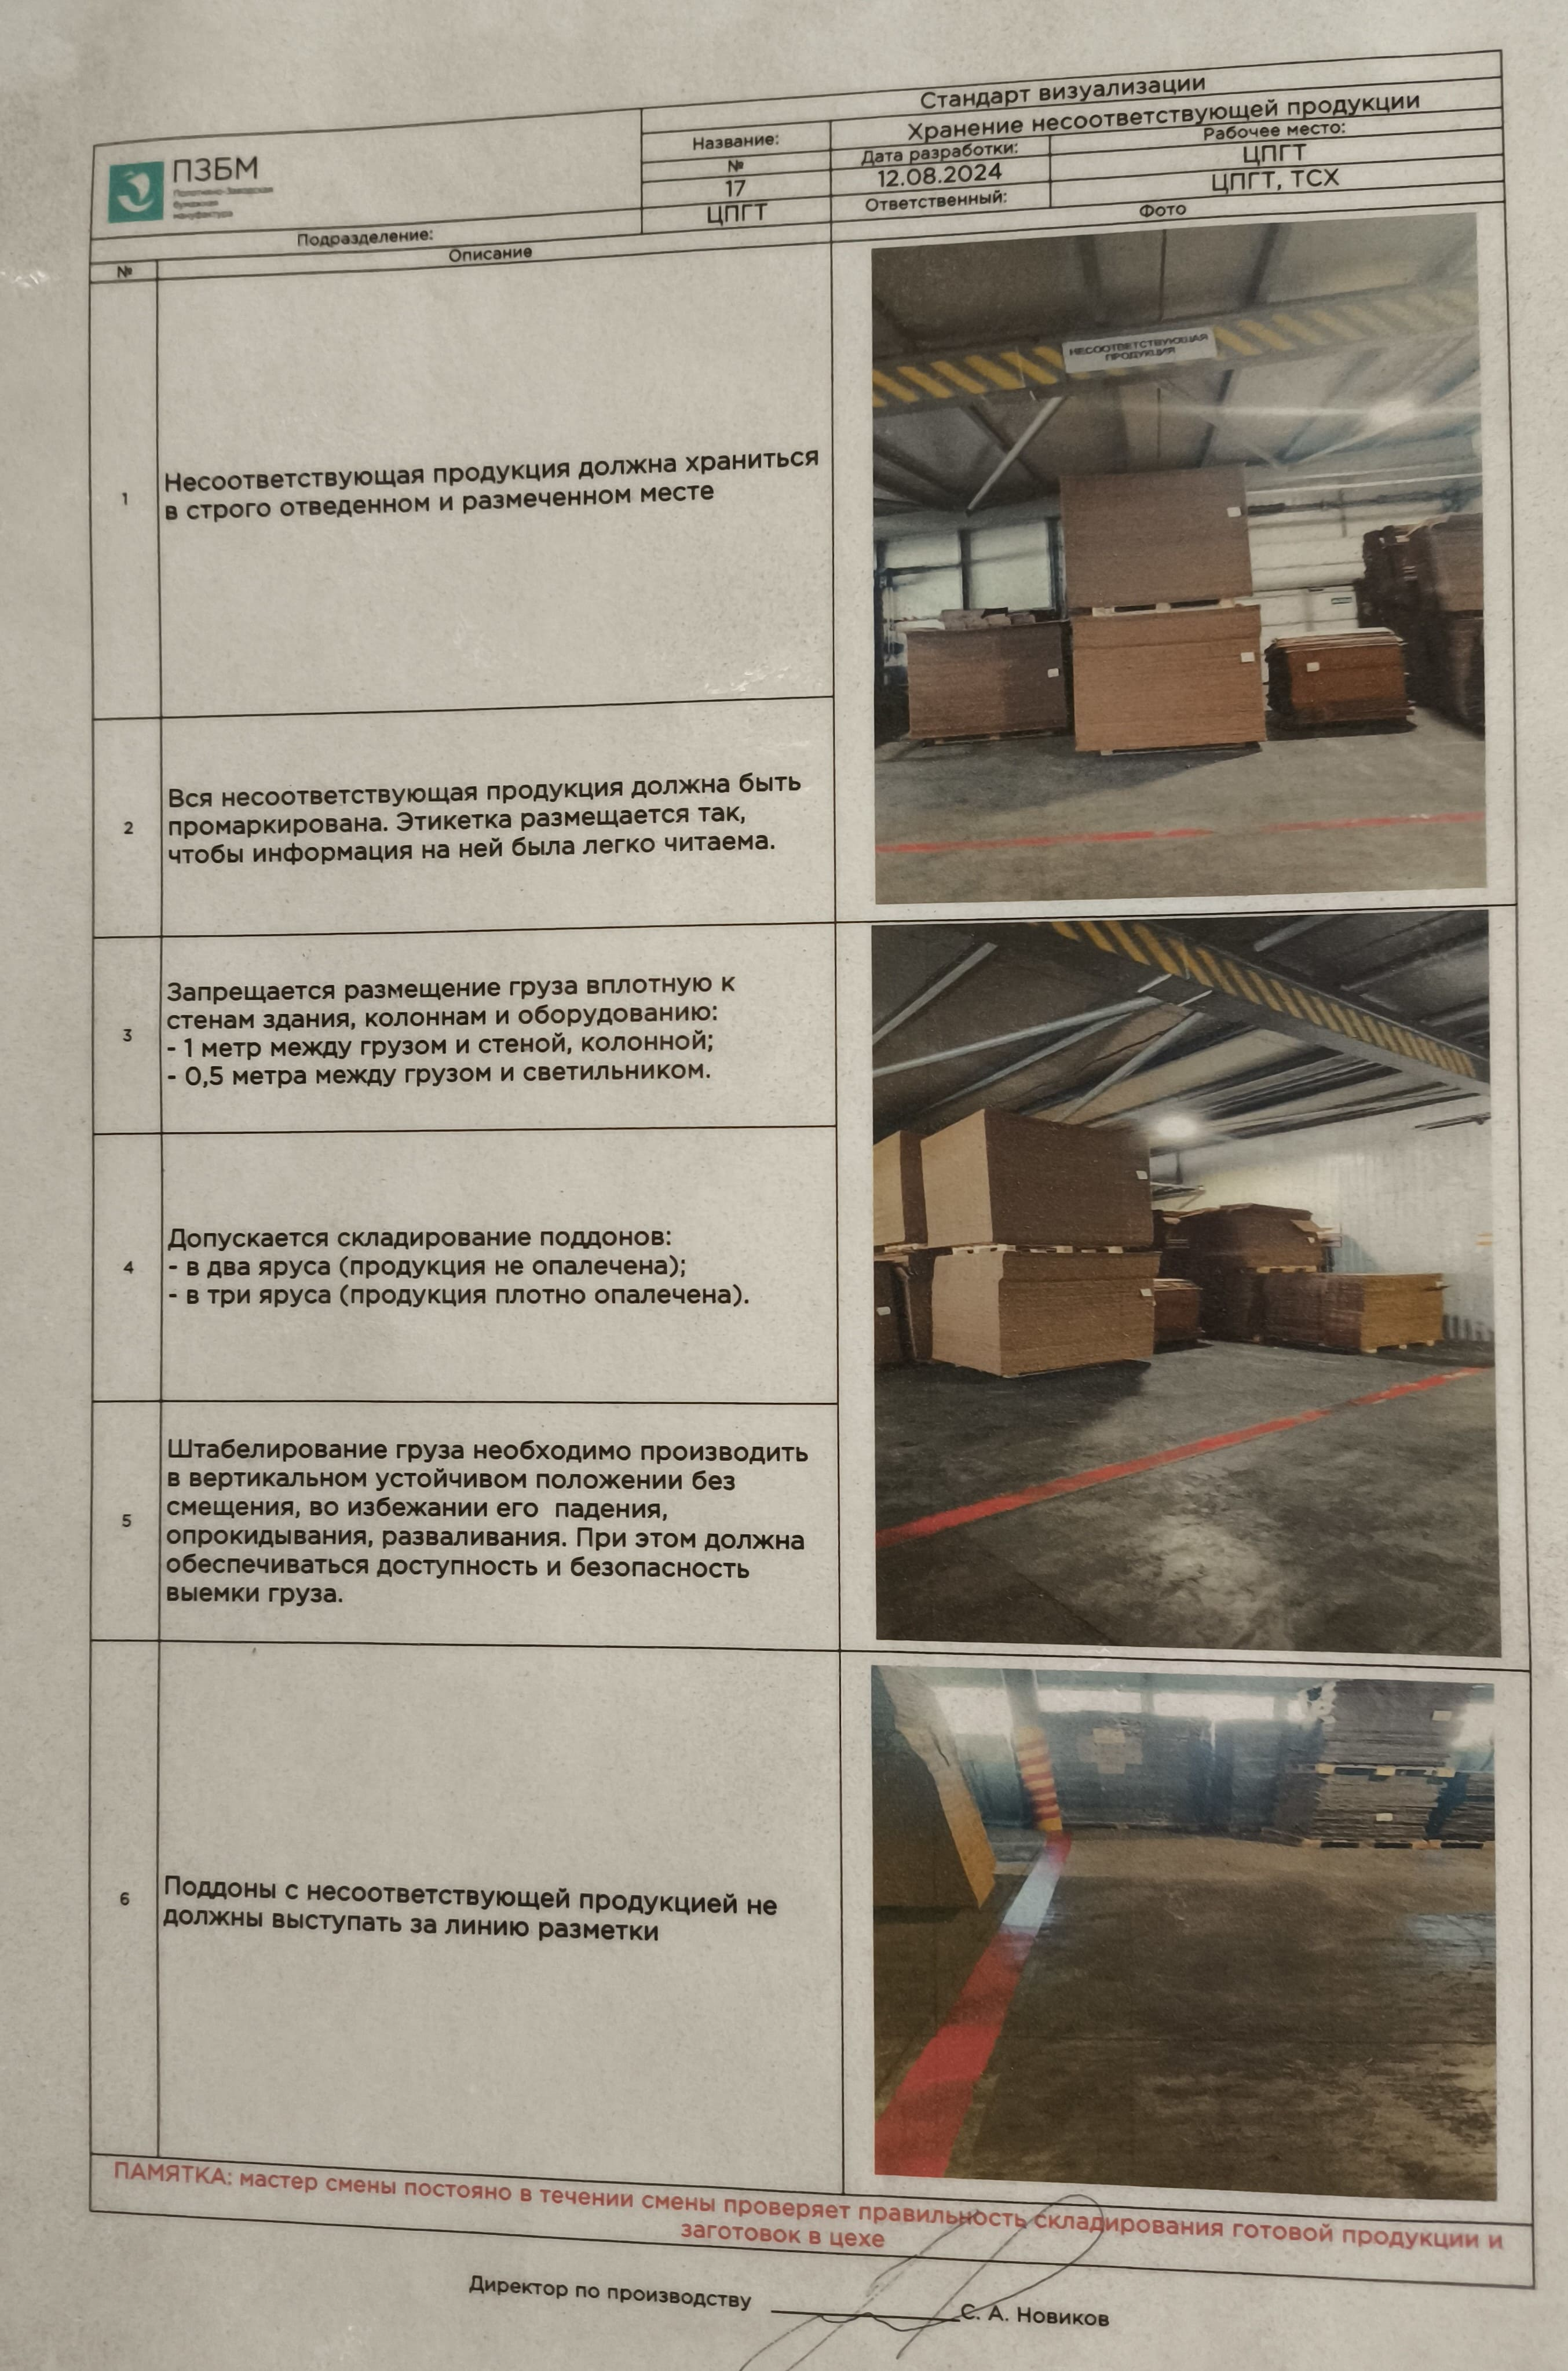
\includegraphics[height=0.9\textheight, keepaspectratio]{Pics/VIII как хранить брак.jpg}
\end{center}
 \caption{Инструкция по хранению брака}
 \label{pic:/VIII как хранить брак}
\end{figure}

\begin{figure}
\begin{center}
 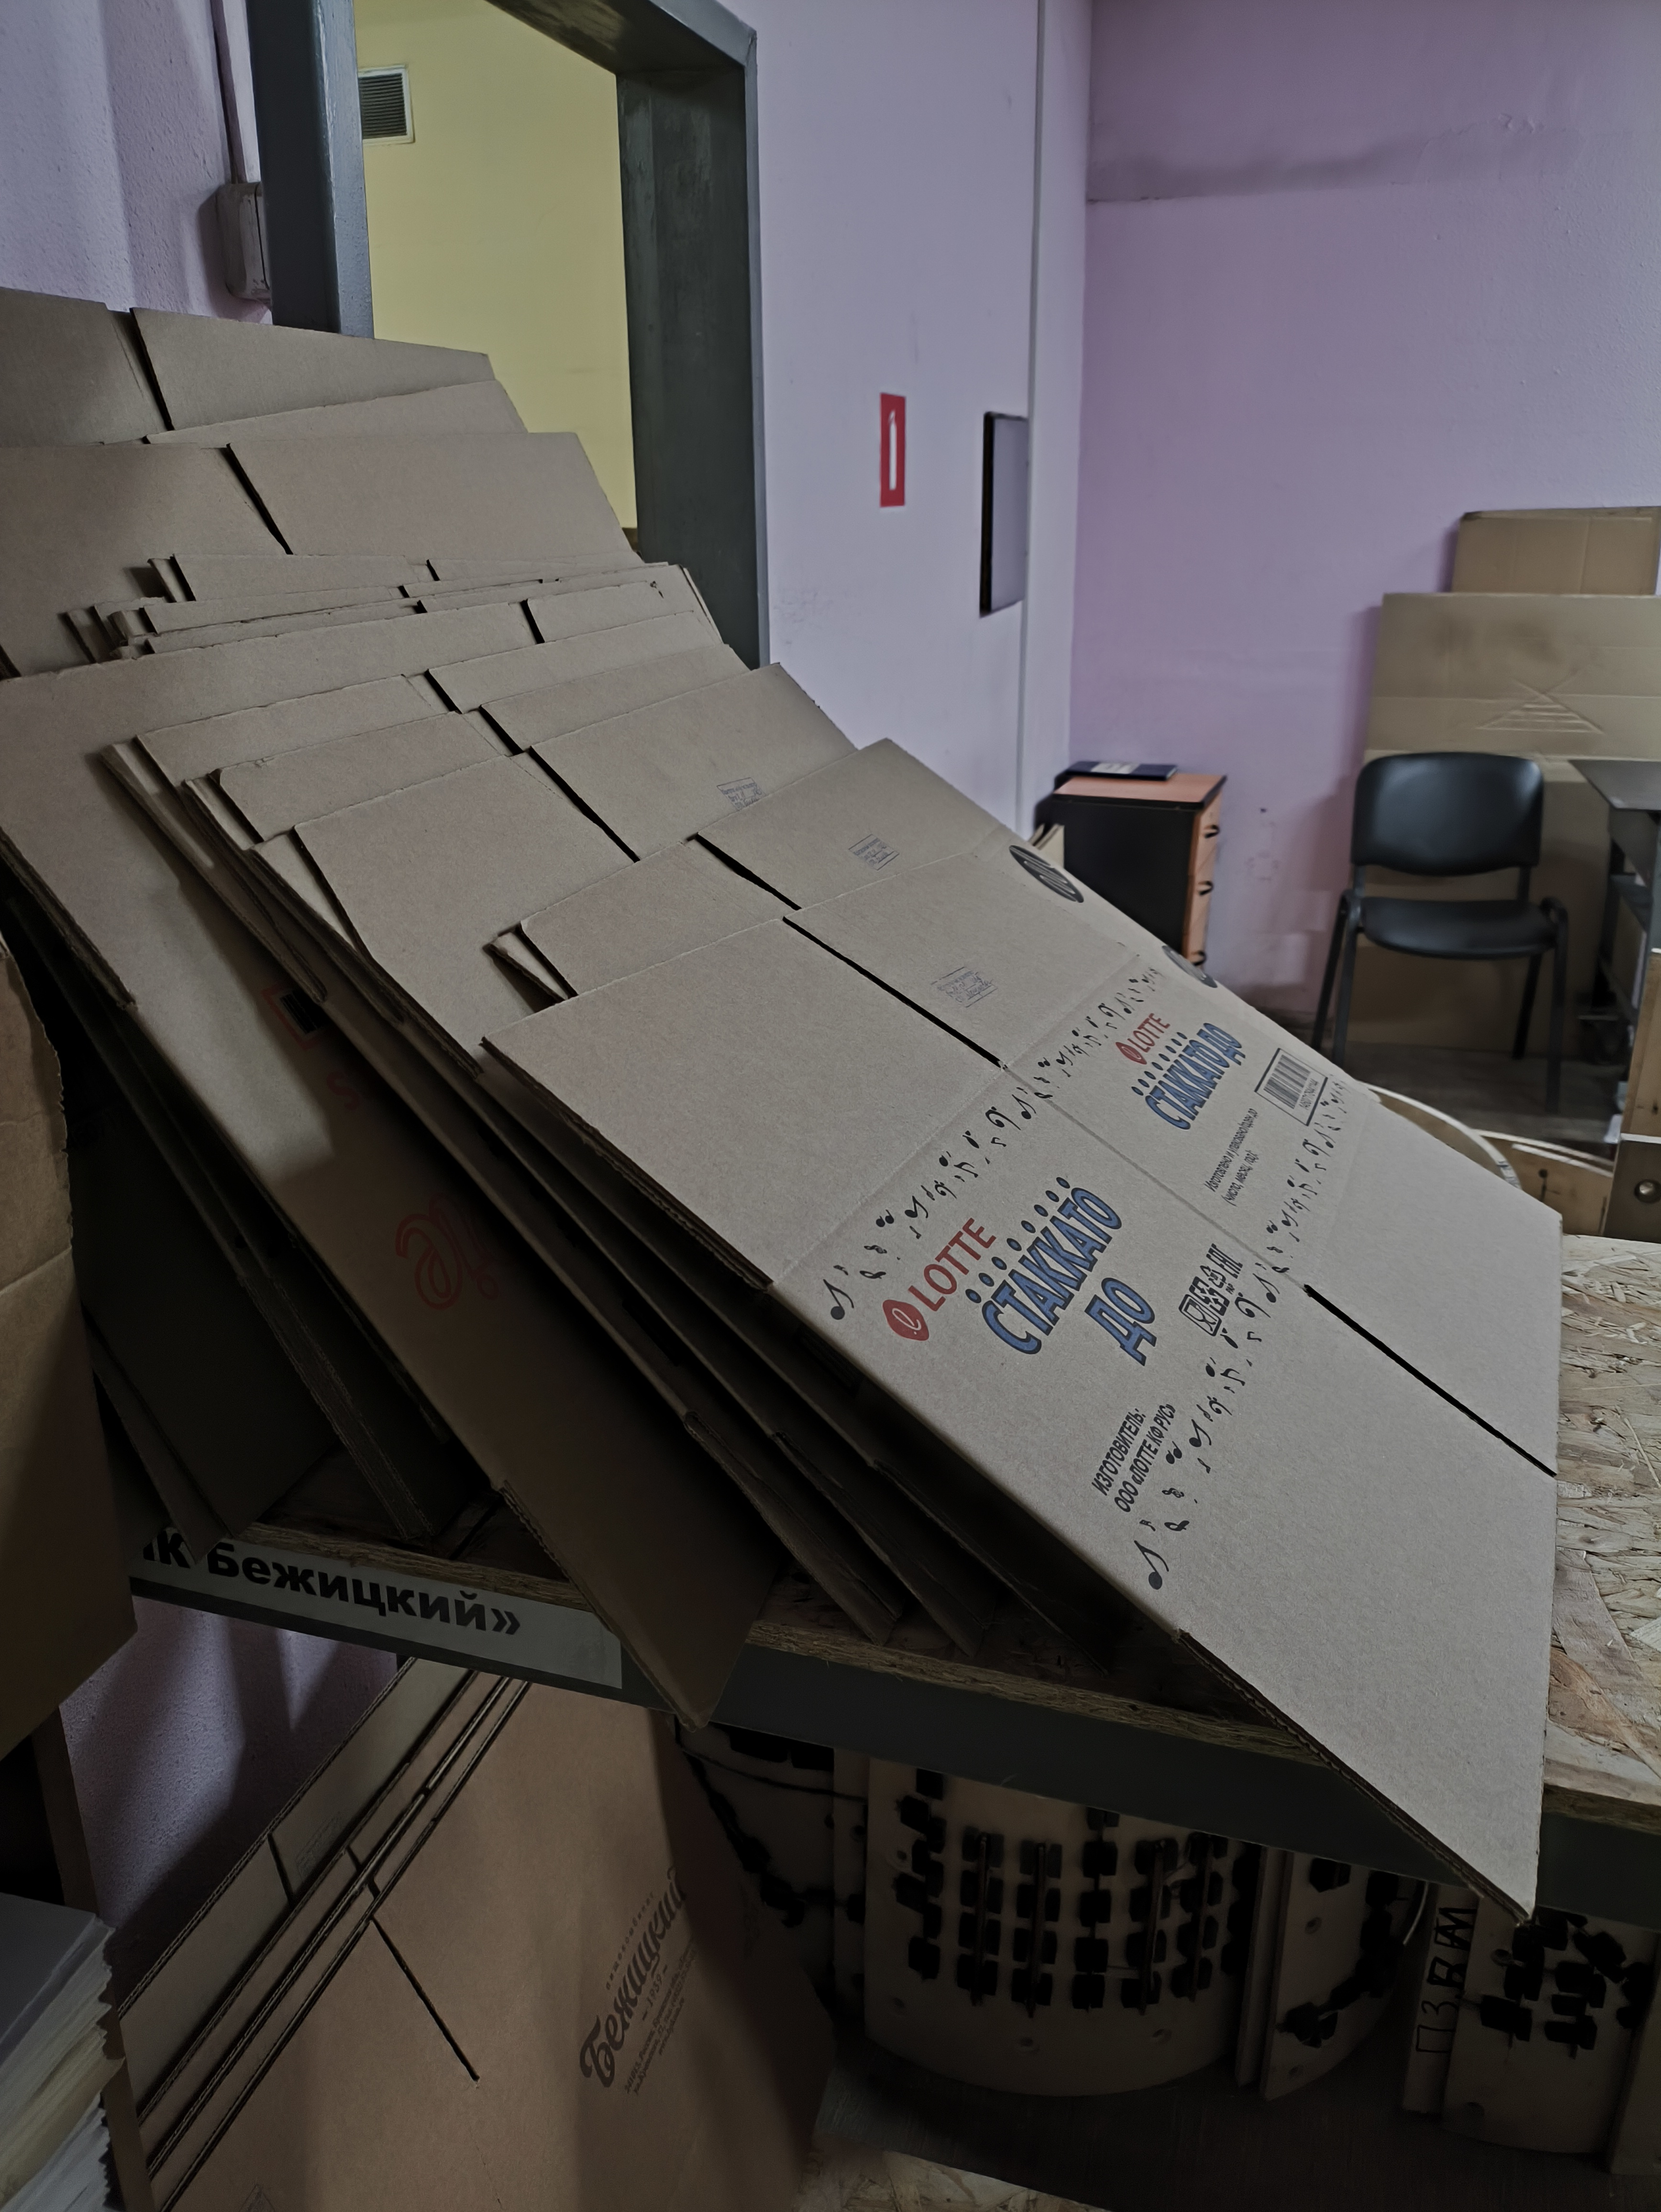
\includegraphics[height=0.9\textheight, keepaspectratio]{Pics/VIIIконтрольныеобразцы.jpg}
\end{center}
 \caption{Контрольные образцы}
 \label{pic:/VIIIконтрольныеобразцы}
\end{figure}

\begin{figure}
\begin{center}
 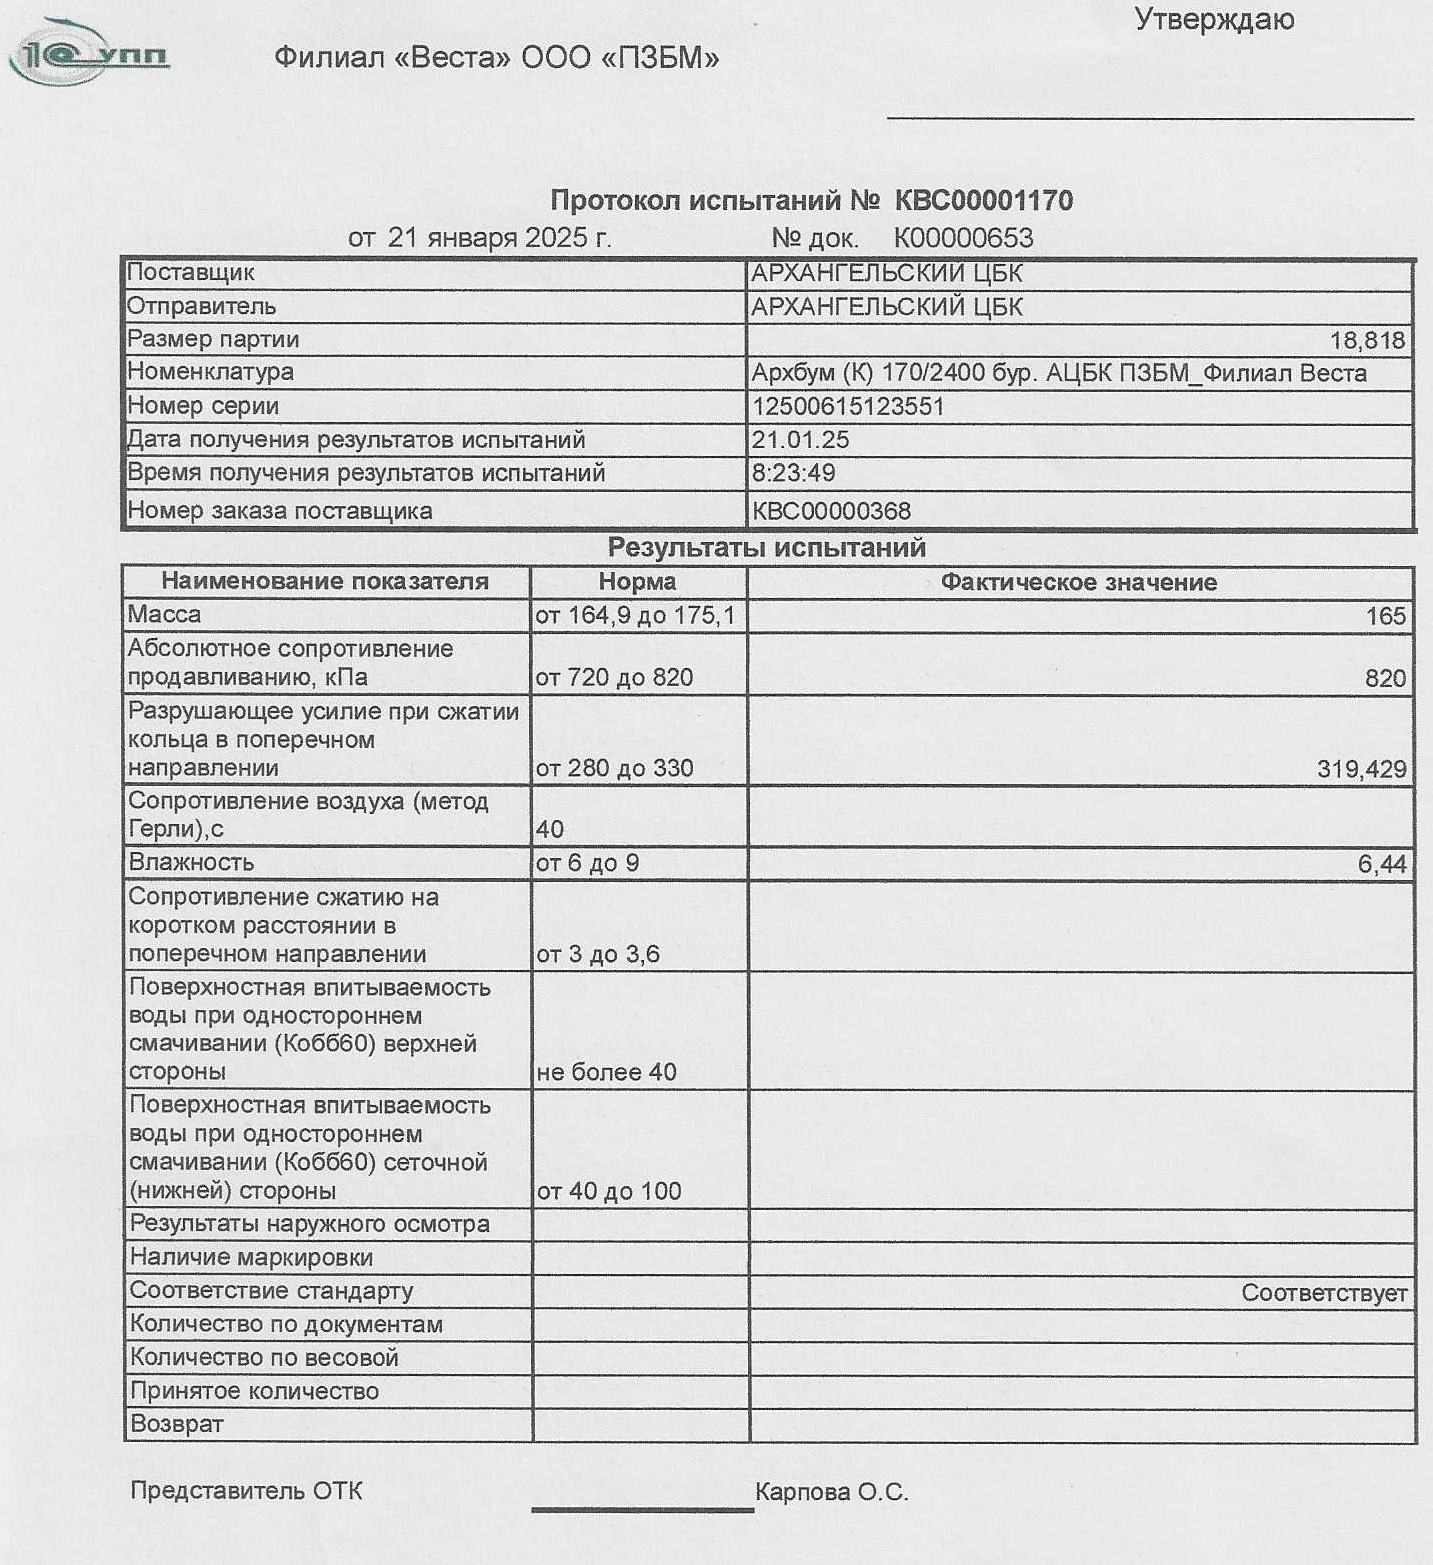
\includegraphics[height=0.7\textheight, keepaspectratio]{Pics/VIII.1.jpg}
\end{center}
 \caption{Протокол испытаний}
 \label{pic:/VIII.1}
\end{figure}

\begin{figure}
\begin{center}
 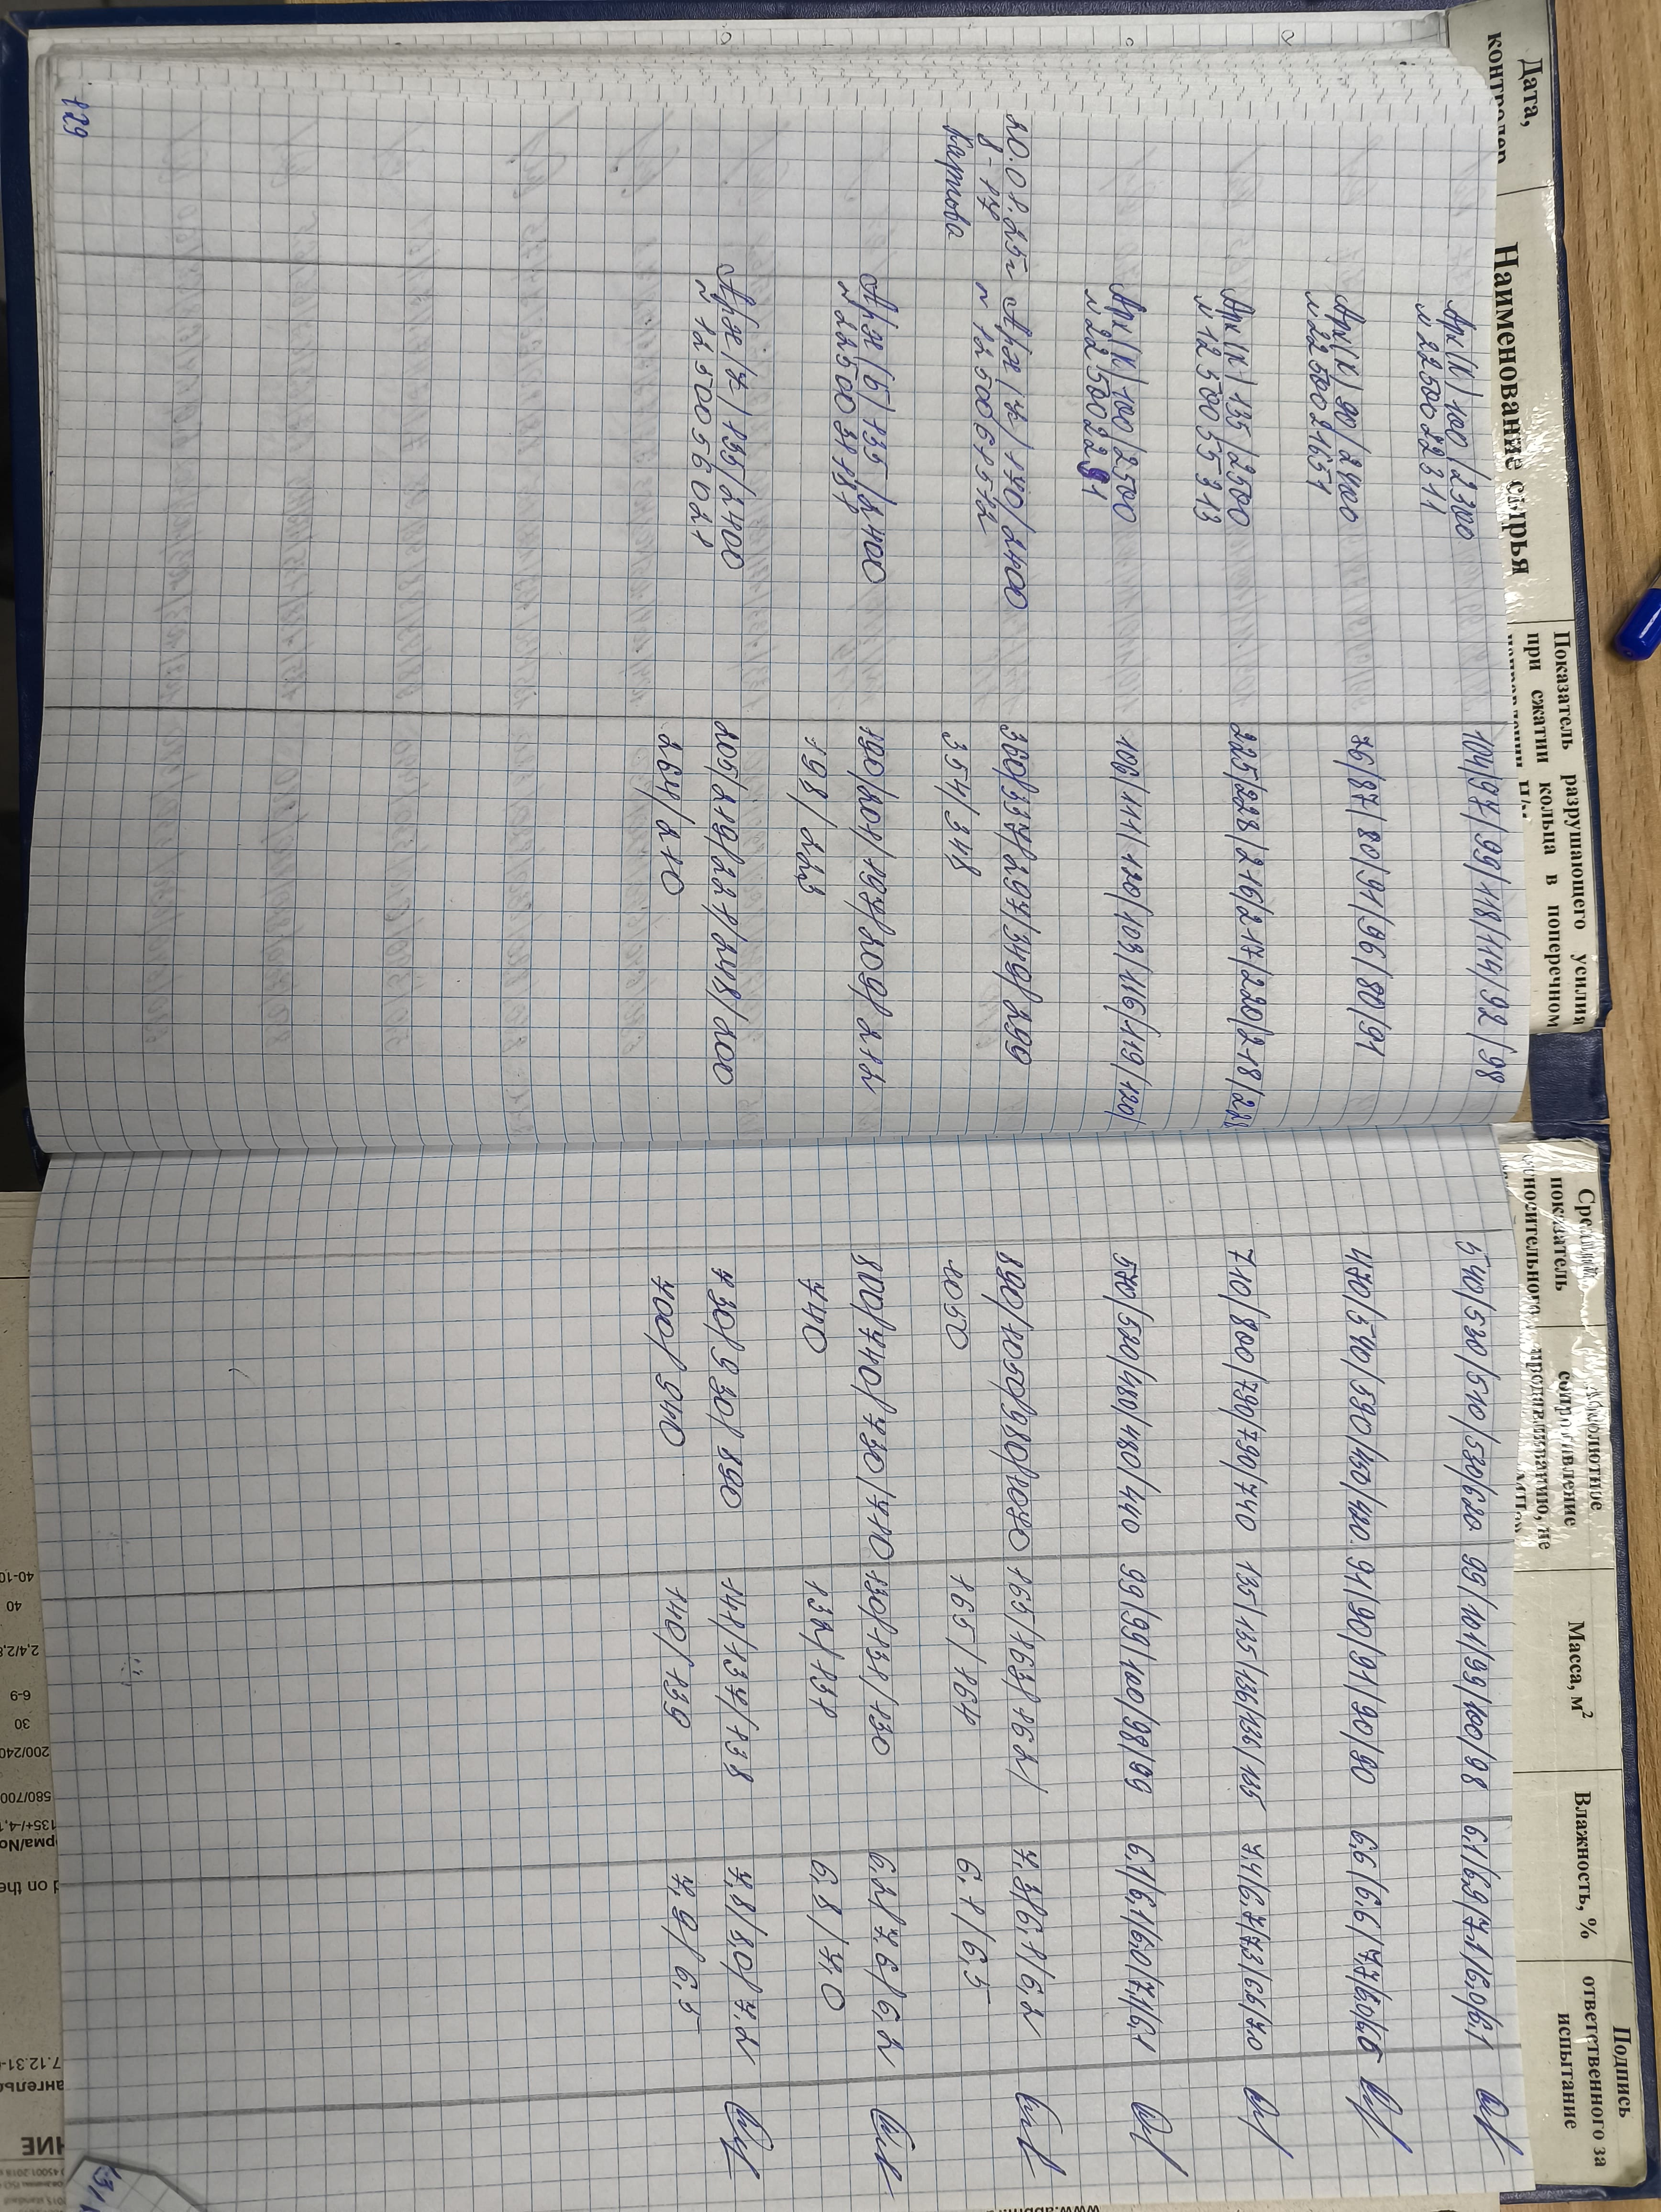
\includegraphics[height=0.9\textheight, angle=180, keepaspectratio]{Pics/VIII анализы сырья.jpg}
\end{center}
 \caption{Журнал входного контроля на сырье}
 \label{pic:/VIII анализы сырья}
\end{figure}



% \begin{figure}
% \begin{center}
%  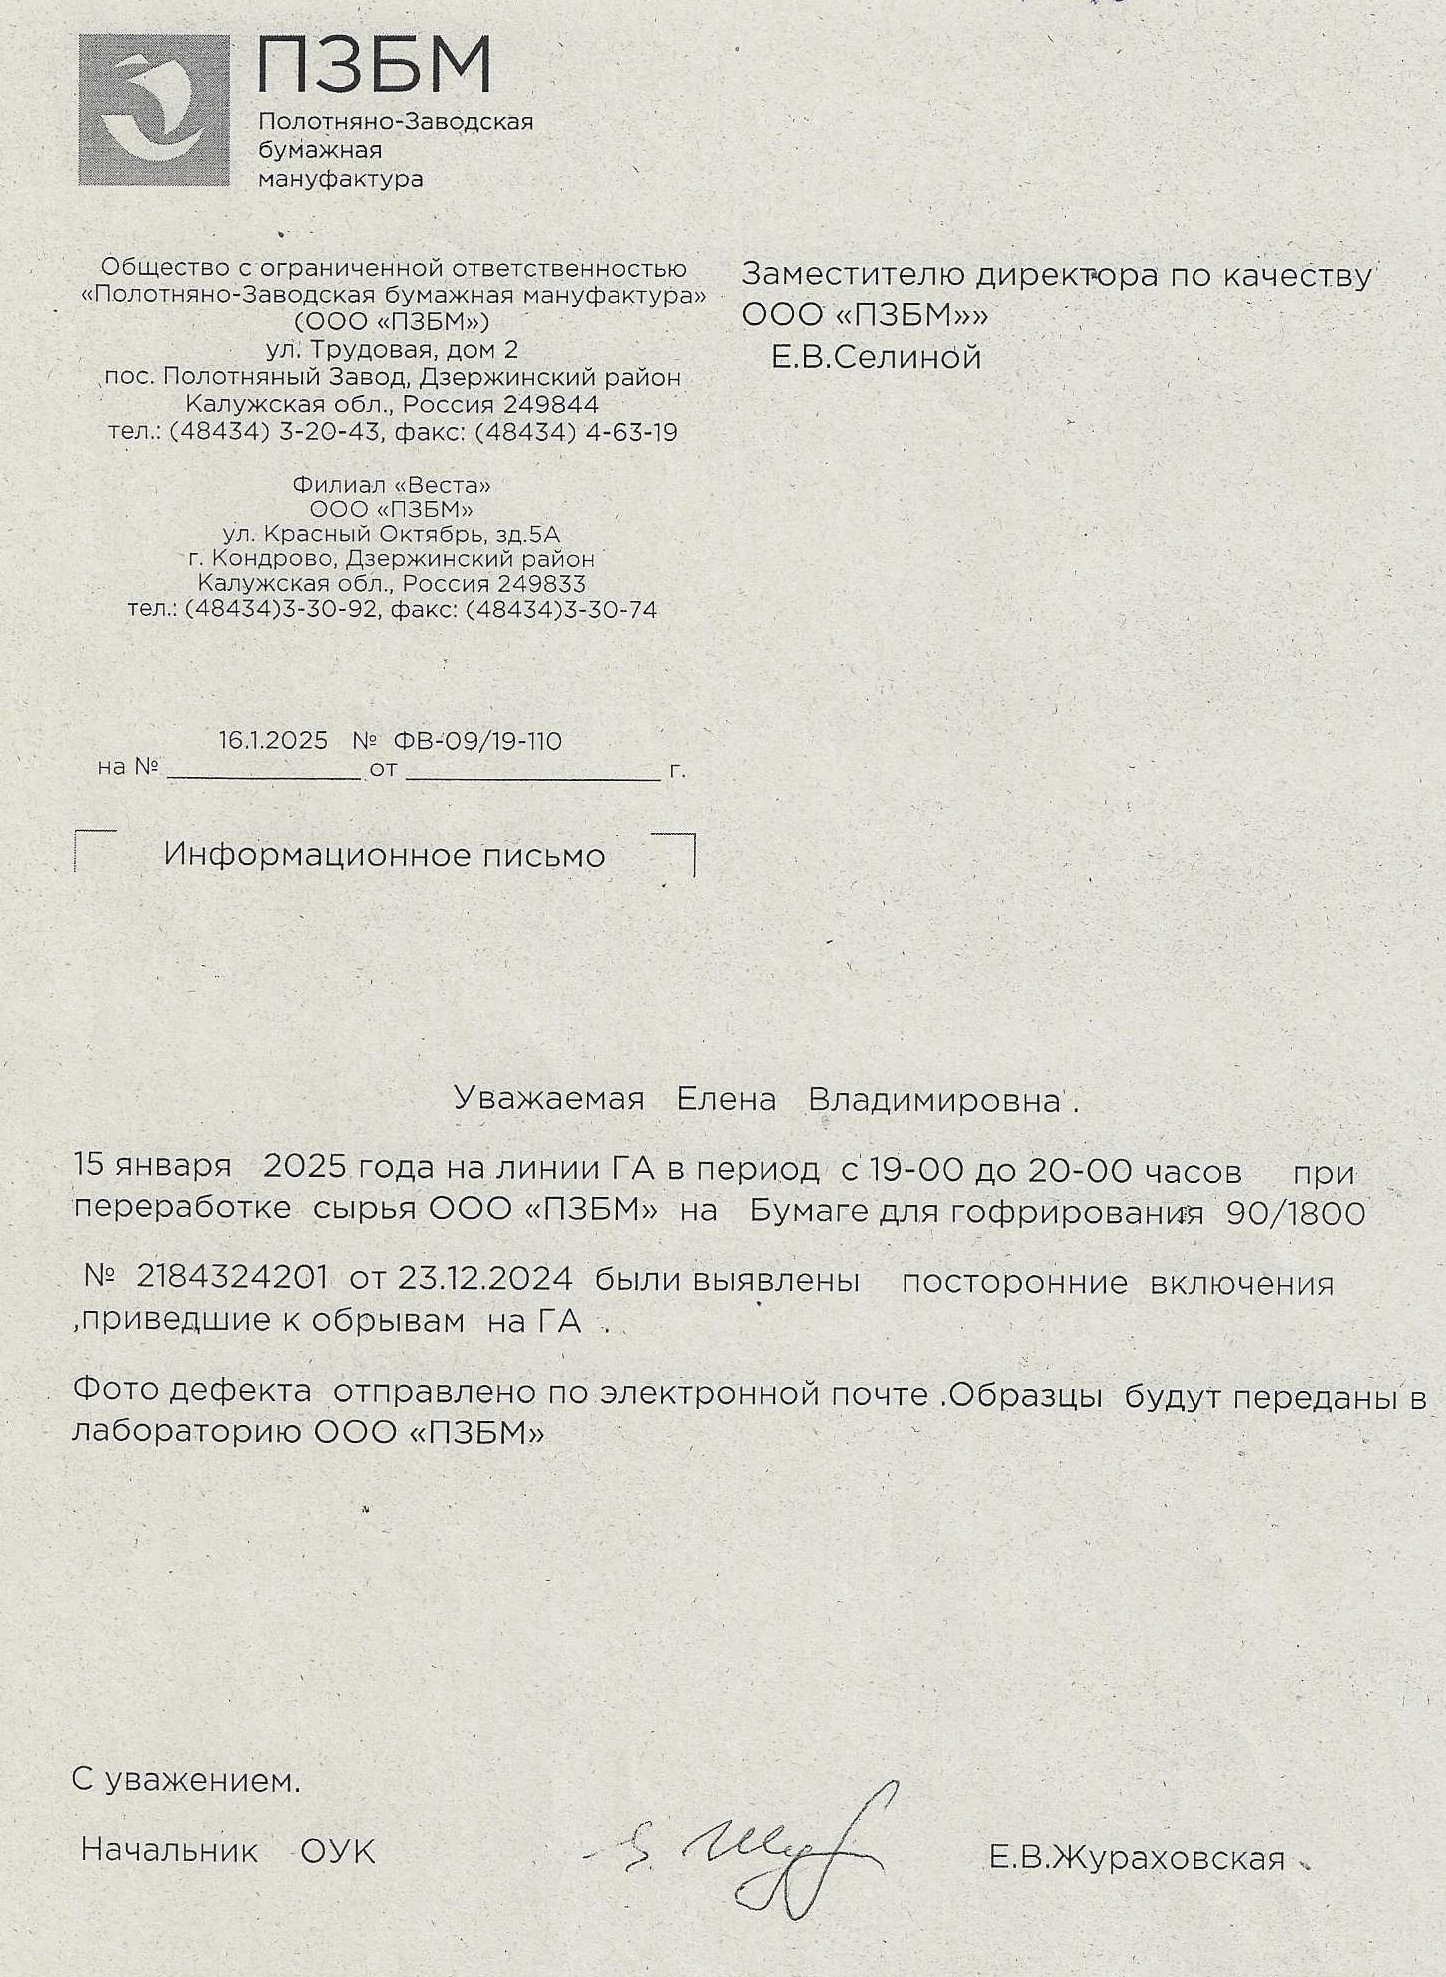
\includegraphics[height=0.9\textheight, keepaspectratio]{Pics/VIII.6.jpg}
% \end{center}
%  \caption{Информационное письмо}
%  \label{pic:/VIII.6}
% \end{figure}

\begin{figure}
\begin{center}
 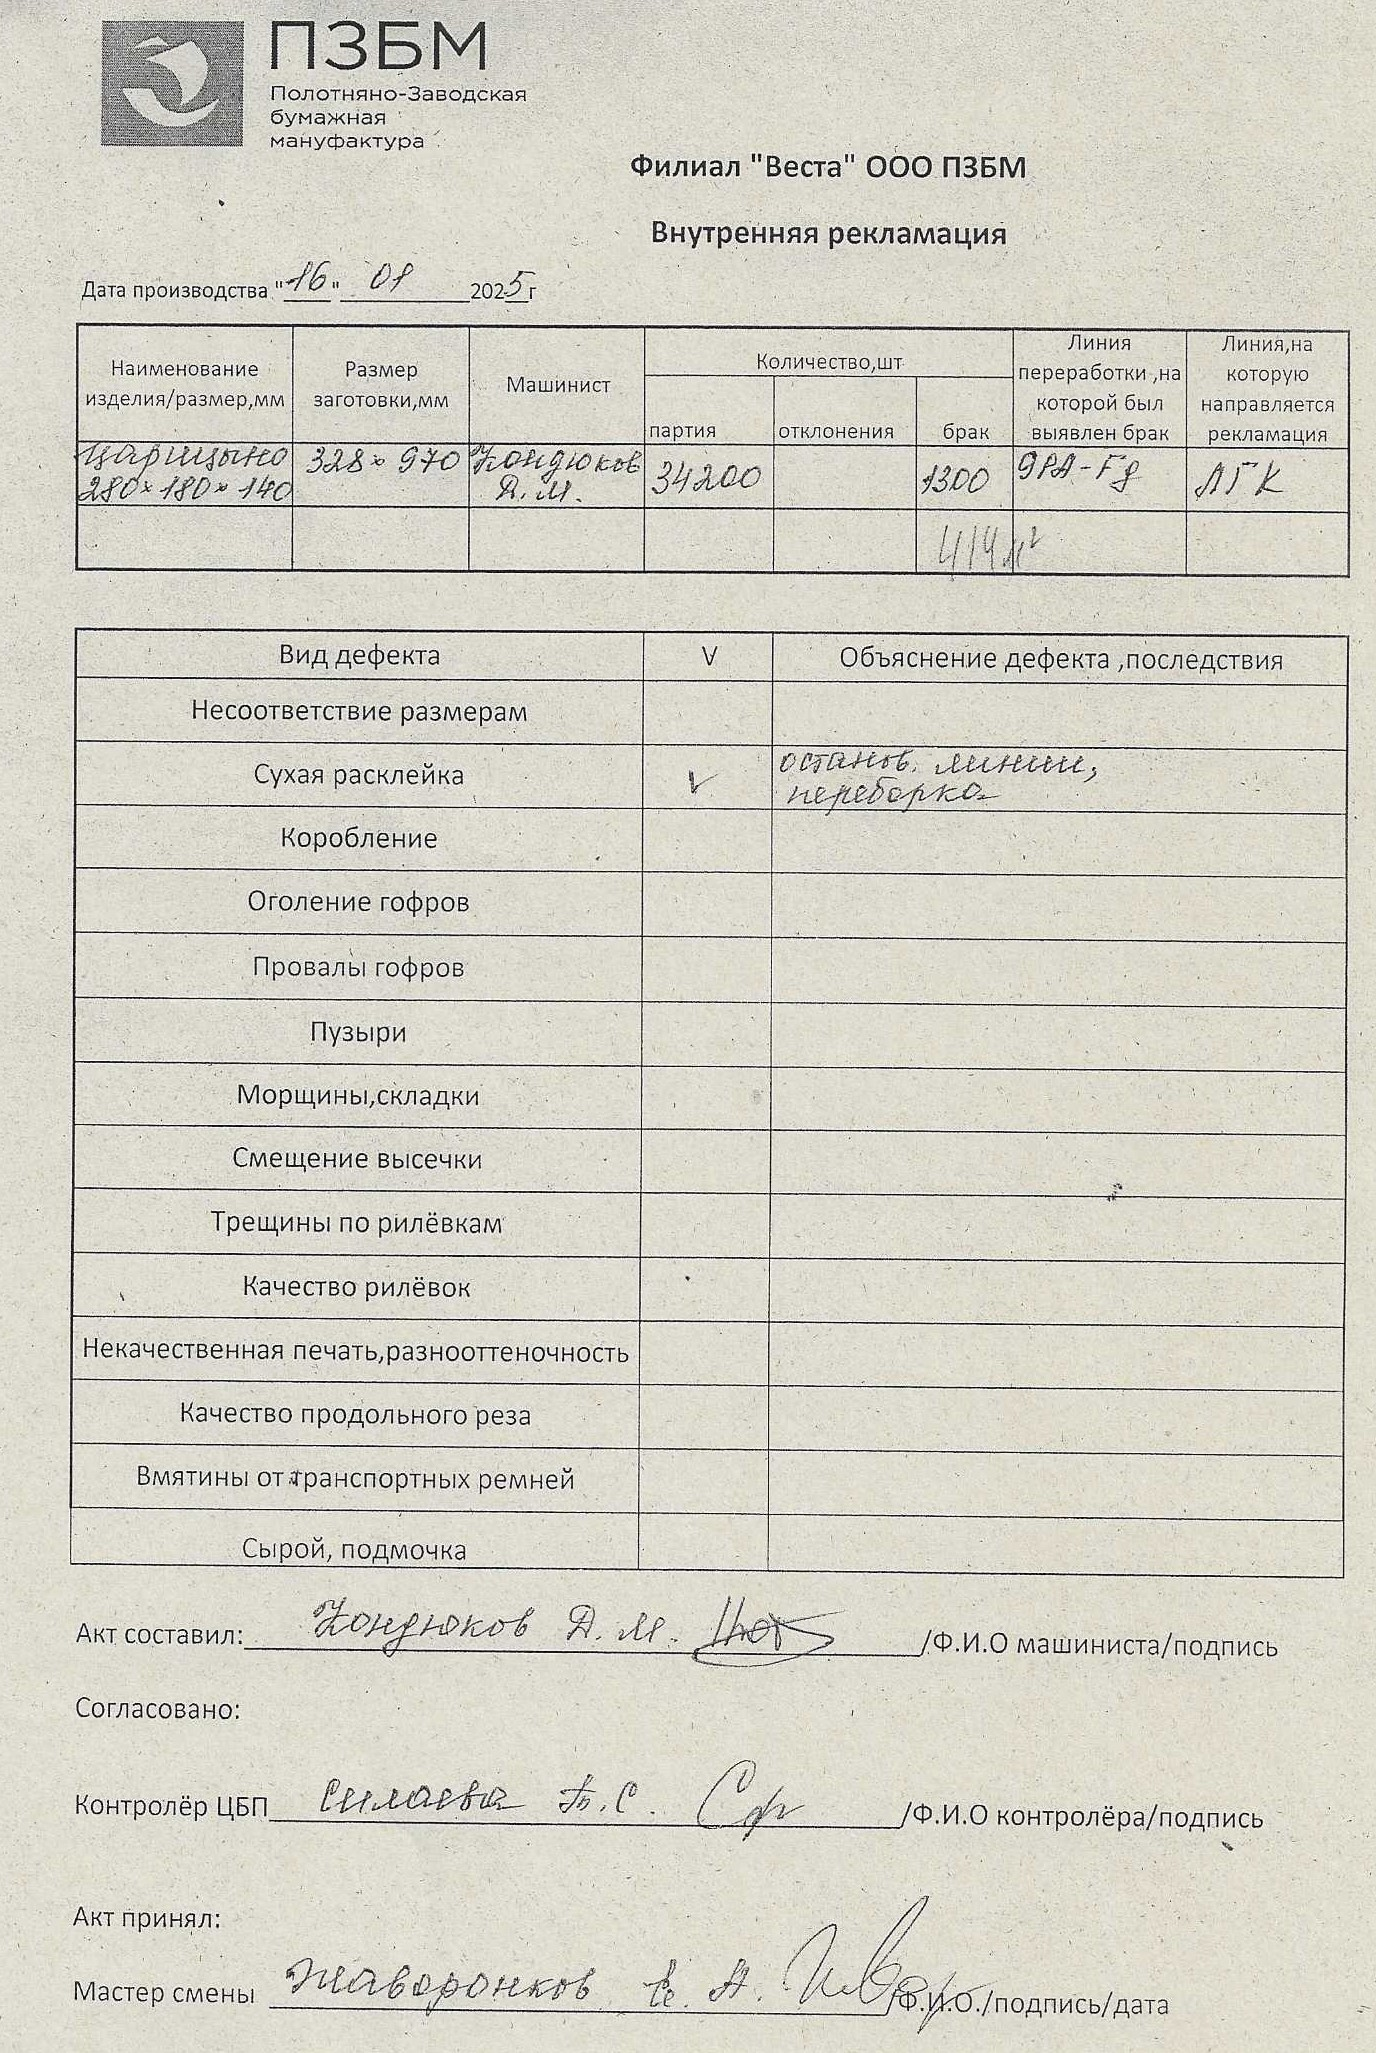
\includegraphics[height=0.9\textheight, keepaspectratio]{Pics/VIII.11.jpg}
\end{center}
 \caption{Внутренняя претензия}
 \label{pic:/VIII.11}
\end{figure}

\begin{figure}
\begin{center}
 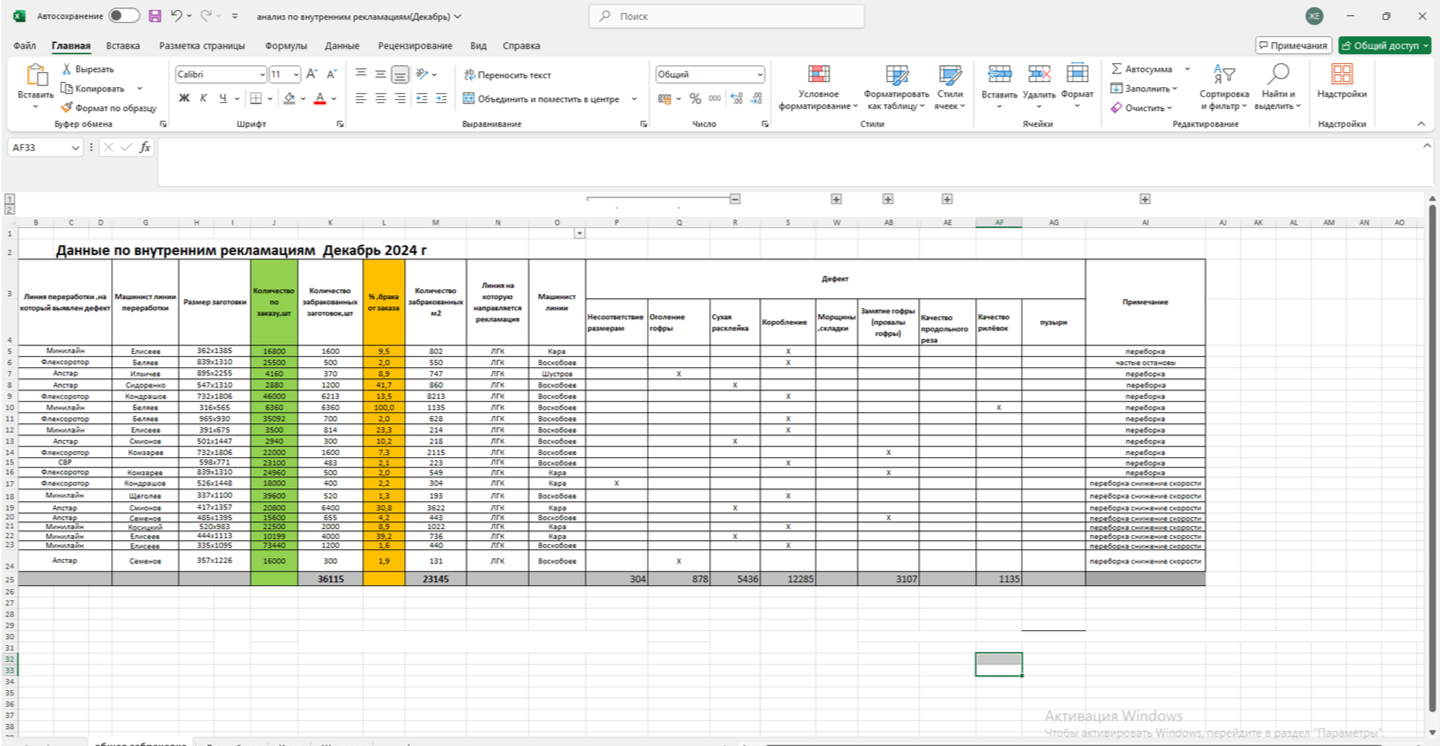
\includegraphics[height=0.35\textheight, keepaspectratio]{Pics/VIIIвнпретензии.png}
\end{center}
 \caption{Статистика по внутренним претензиям}
 \label{pic:/VIIIвнпретензии}
\end{figure}

\begin{figure}
\begin{center}
 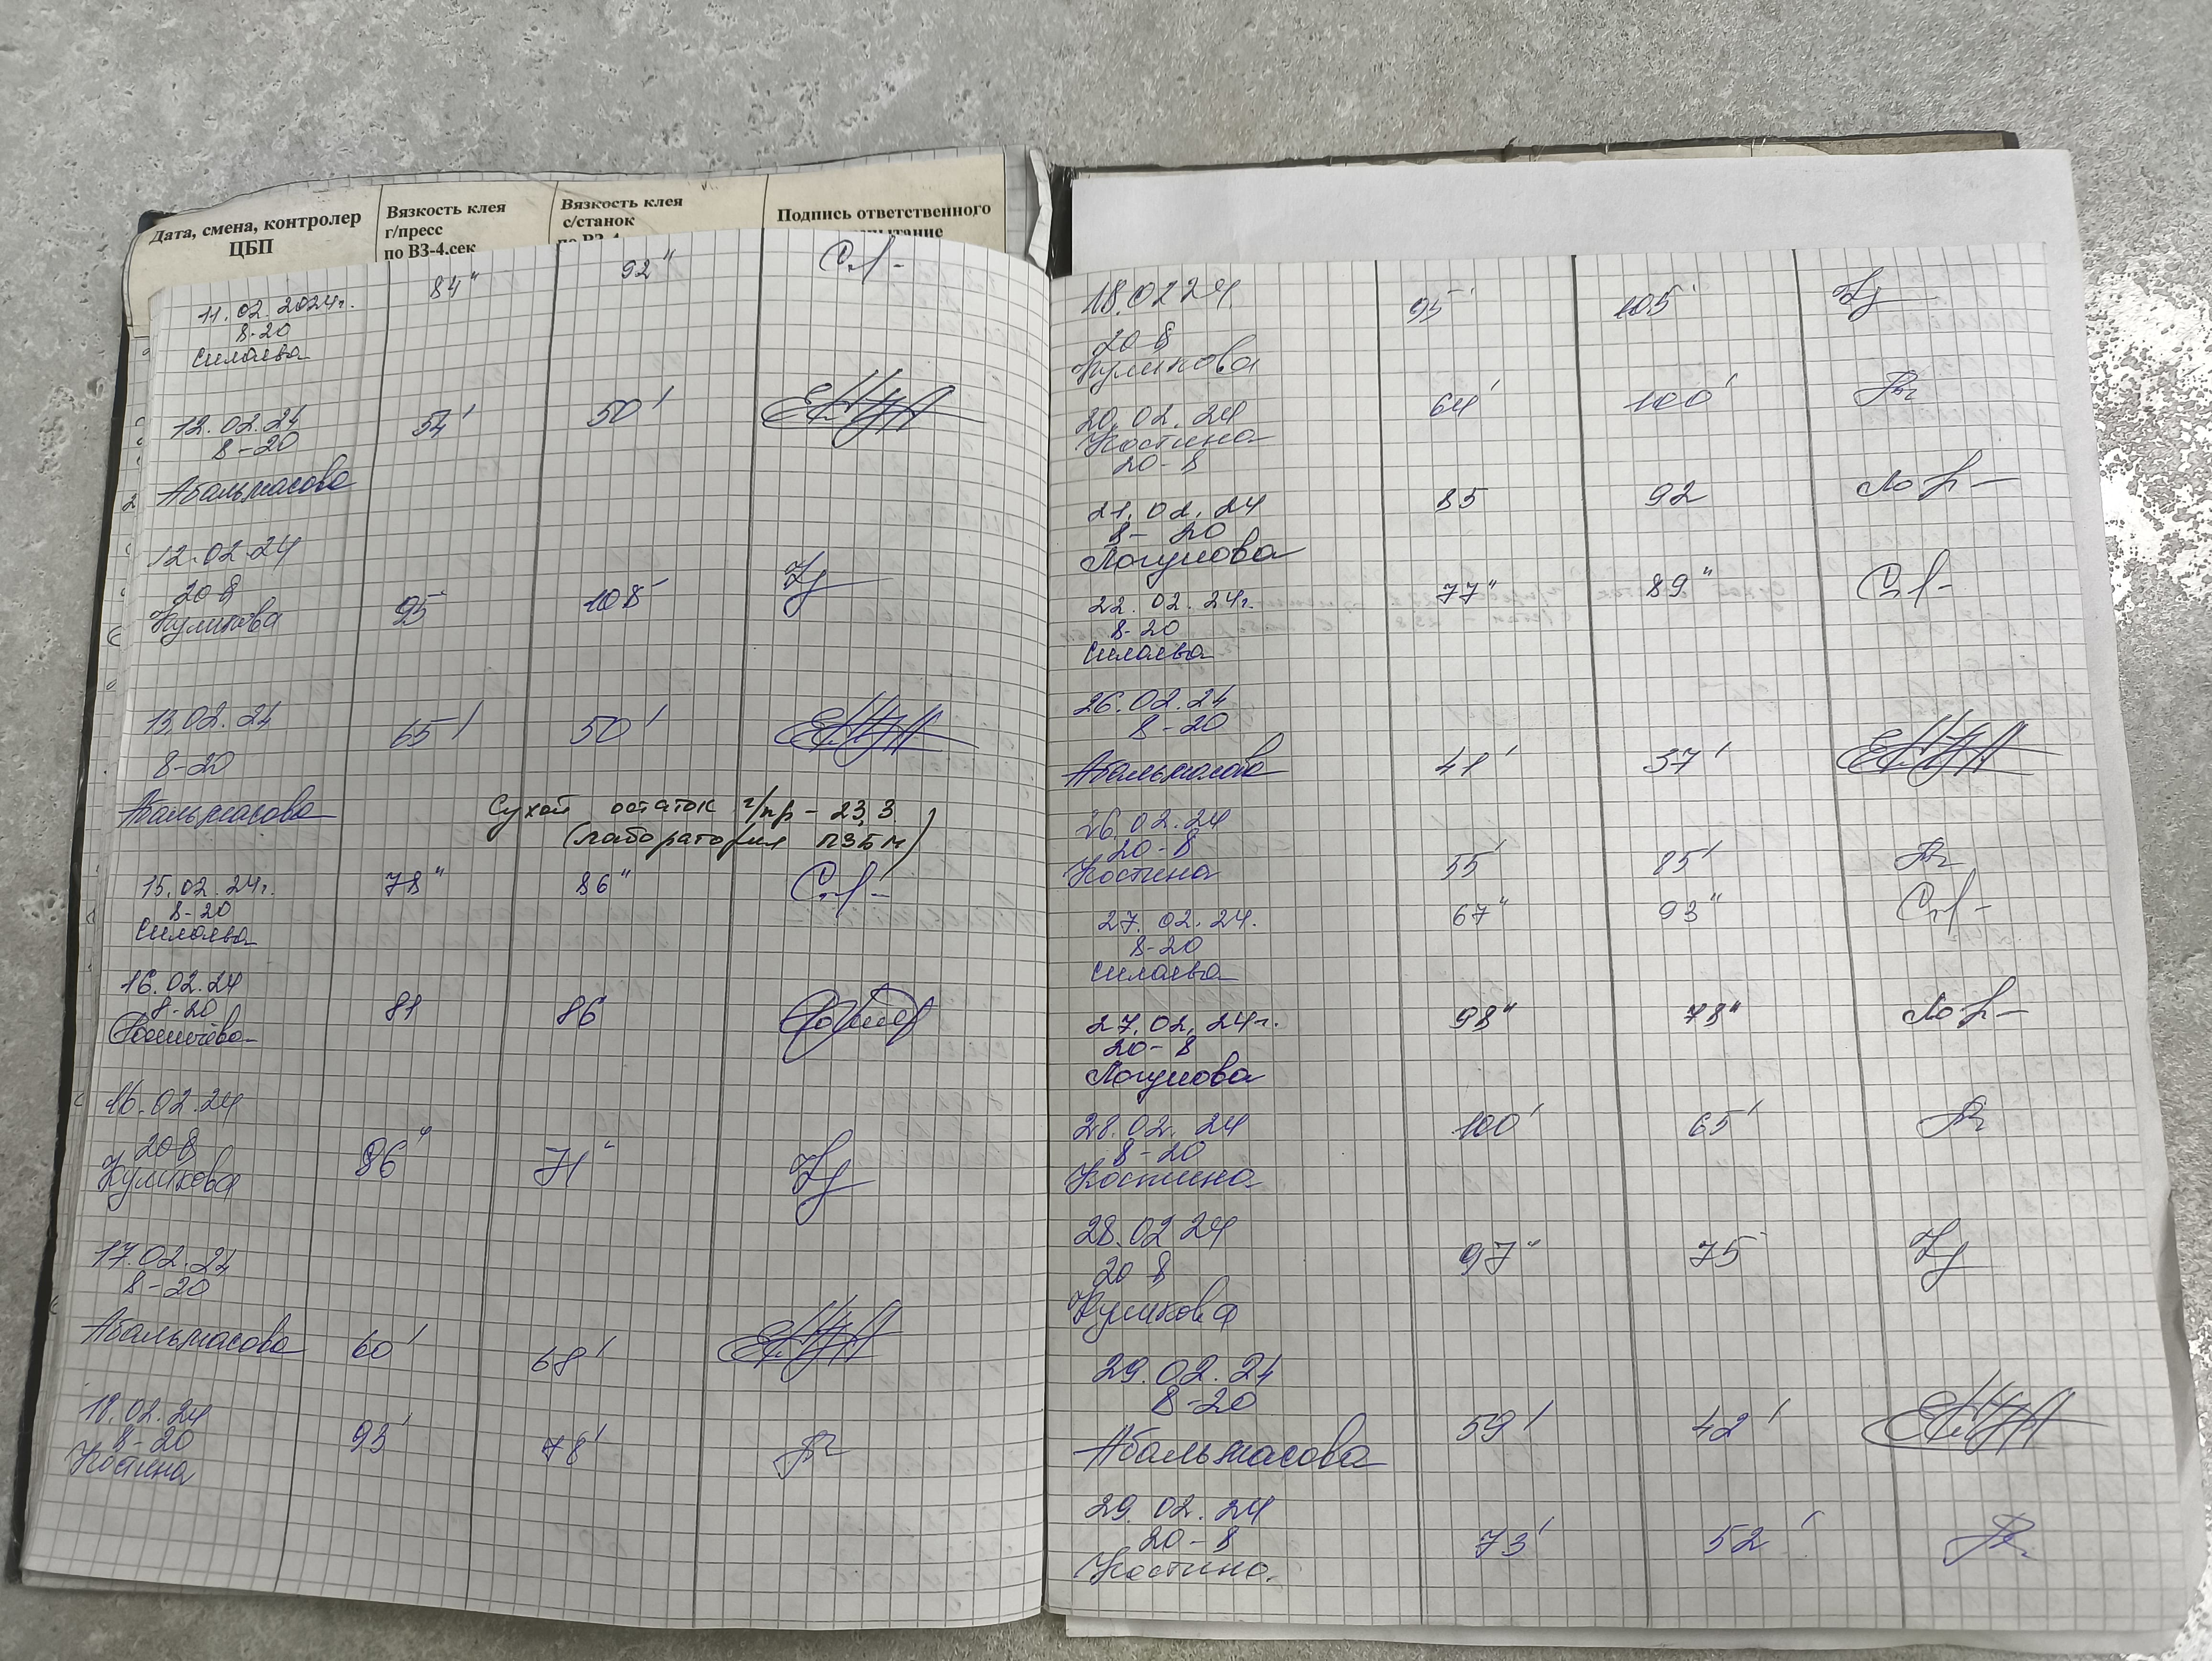
\includegraphics[height=0.45\textheight, keepaspectratio]{Pics/VIII журнал клея.jpg}
\end{center}
 \caption{Журнал вязкости клея}
 \label{pic:/VIII журнал клея}
\end{figure}

\begin{figure}
\begin{center}
 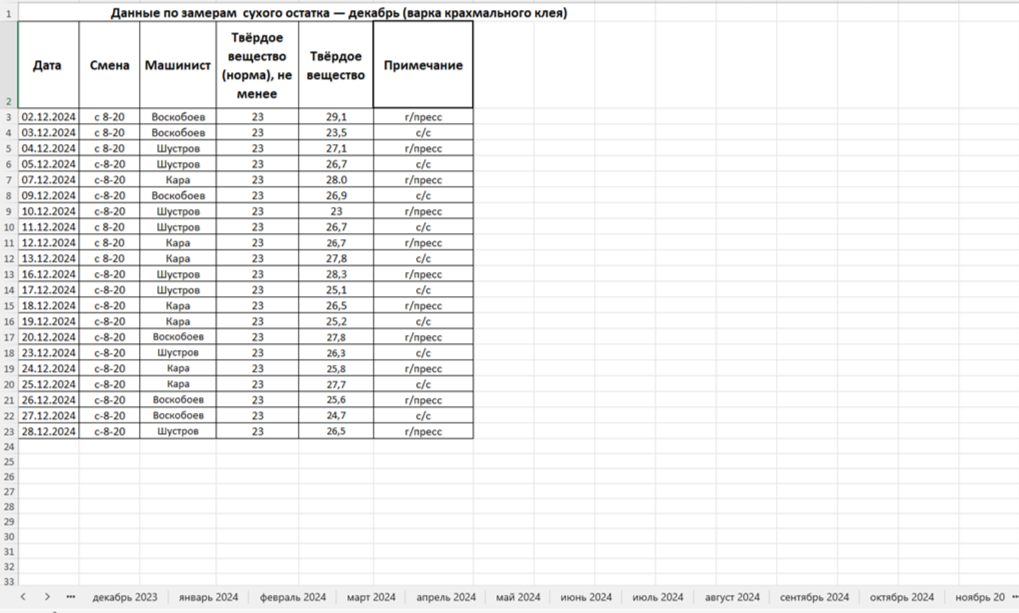
\includegraphics[height=0.4\textheight, keepaspectratio]{Pics/VIIIсухойостаток.png}
\end{center}
 \caption{Отчеты по измерению сухого остатка}
 \label{pic:/VIIIсухойостаток}
\end{figure}

\begin{figure}
\begin{center}
 \includegraphics[height=0.45\textheight, keepaspectratio]{Pics/VIIIлаборатория.jpg}
\end{center}
 \caption{Лаборатория}
 \label{pic:/VIIIлаборатория}
\end{figure}

\begin{figure}
\begin{center}
 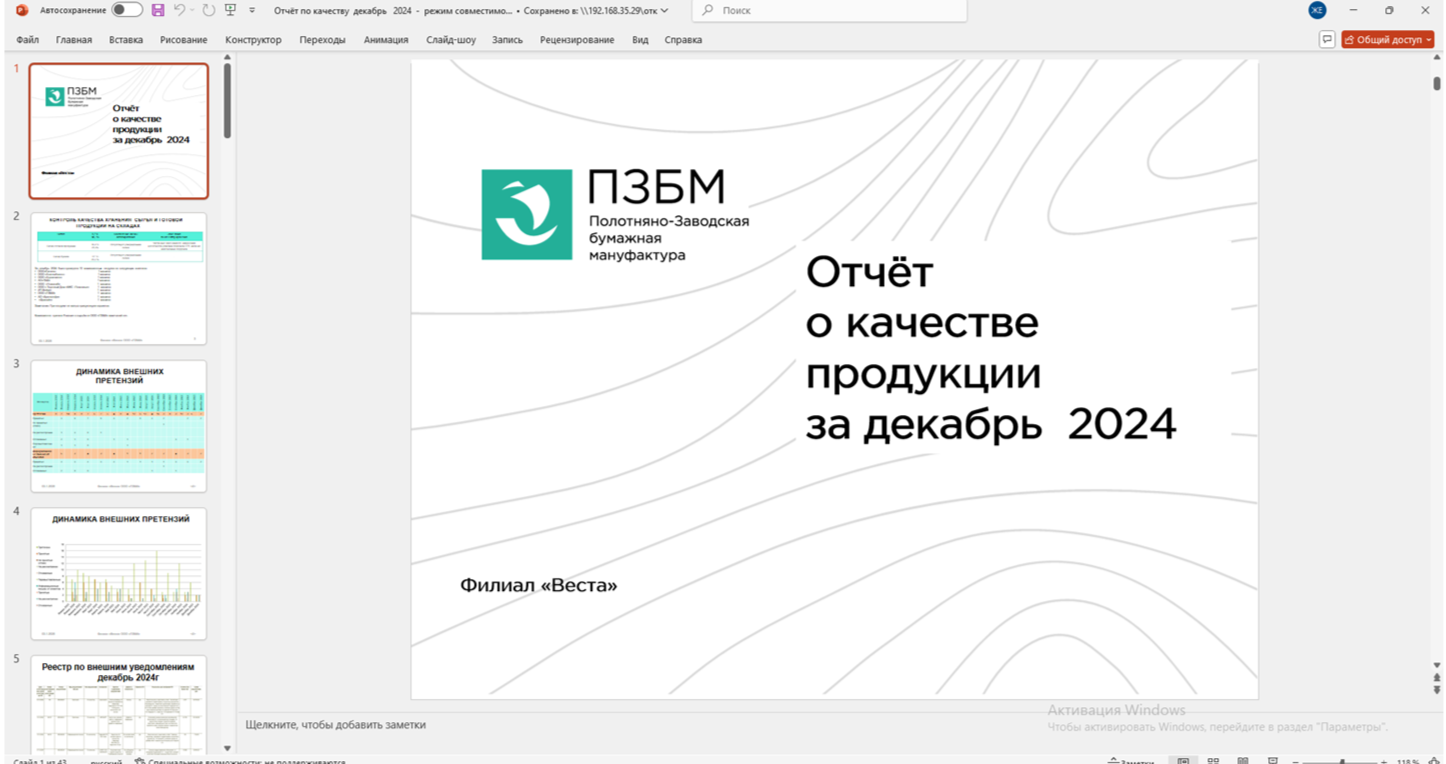
\includegraphics[height=0.35\textheight, keepaspectratio]{Pics/VIIIкачество.png}
\end{center}
 \caption{Презентация по качеству}
 \label{pic:/VIIIкачество}
\end{figure}

\begin{figure}
\begin{center}
 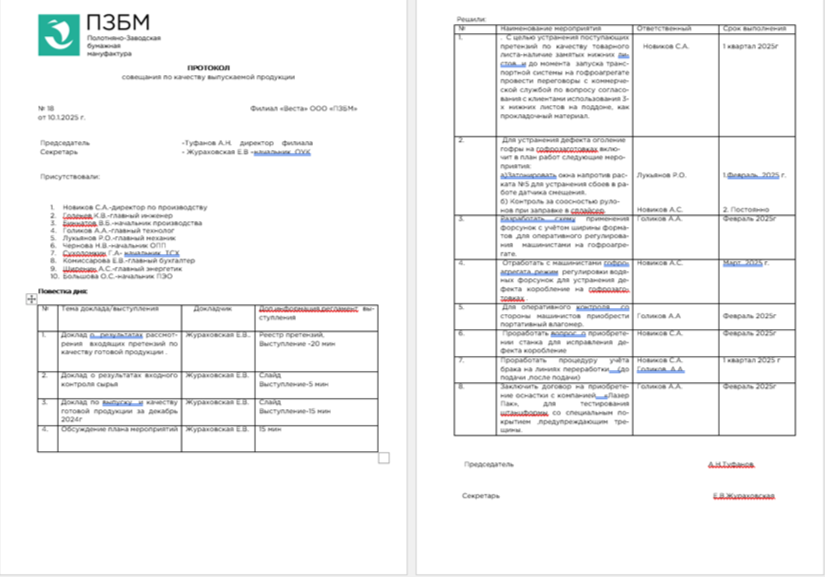
\includegraphics[height=0.42\textheight, keepaspectratio]{Pics/VIIIсовещание.png}
\end{center}
 \caption{Протокол совещания по качеству продукции}
 \label{pic:/VIIIсовещание}
\end{figure}
\clearpage
\ifx \notincludehead\undefined
\normalsize
\end{document}
\fi